\documentclass[phd]{ppgccufmg} % ou [msc] para dissertações
% de mestrado. Para propostas ou
% projetos, usar [phd,project],
% [msc,proposal], etc.

\usepackage[english]{babel}
\usepackage[T1]{fontenc}
\usepackage[utf8x]{inputenc}
\usepackage{type1ec}

\usepackage{graphicx}
\usepackage[square]{natbib} % permite citações naturalmente integradas ao texto



%\usepackage{array}
\usepackage{subcaption}

\usepackage{xspace}

\newcommand{\mcode}[1]{$\mathtt{#1}$} 
\newcommand{\quotes}[1]{``#1''}
\newcommand{\margin}[0]{\\[-0.3cm]}

\newcommand{\totalProjects}[0]{748\xspace}
\newcommand{\activeProjects}[0]{471\xspace}
\newcommand{\activeProjectsPercentage}[0]{63\%}
\newcommand{\refactoredProjects}[0]{285\xspace}
\newcommand{\refactoredProjectsPercentage}[0]{38\%}
\newcommand{\studiedProjects}[0]{124\xspace}
\newcommand{\studiedProjectsPercentage}[0]{17\%}
\newcommand{\studiedDevelopers}[0]{222\xspace}
\newcommand{\toolName}[0]{RefactoringMiner\xspace}
\newcommand{\refactoringTypes}[0]{12\xspace}
\newcommand{\totalMotivationThemes}[0]{44\xspace}
\newcommand{\detectedRefactorings}[0]{2,241\xspace}
\newcommand{\studiedRefactorings}[0]{463\xspace}
\newcommand{\commitsWithTruePositiveRefactoring}[0]{539\xspace}
\newcommand{\commitsWithDetectedRefactoring}[0]{729\xspace}
\newcommand{\commitsWithRefactoringAndResponse}[0]{222\xspace} % should be equal to variable studiedDevelopers


\usepackage[english,bookmarks=true,bookmarksnumbered=true,linktocpage,colorlinks=true,citecolor=black,urlcolor=black,linkcolor=black,filecolor=black]{hyperref}

\usepackage{minibar}

\usepackage{multicol}


\usepackage[cmex10]{amsmath}
\usepackage{amssymb}


\DeclareMathOperator{\rmname}{name}
\DeclareMathOperator{\rmcont}{\pi}
\DeclareMathOperator{\rmsig}{sig}
\DeclareMathOperator{\rmsub}{subtype}
\DeclareMathOperator{\rmsuper}{supertype}
\DeclareMathOperator{\rmsubsuper}{subOrSuper}
\DeclareMathOperator{\rmtype}{type}
\DeclareMathOperator{\rmsim}{sim}
\DeclareMathOperator{\rmsimu}{sim_{p}}
\DeclareMathOperator{\rmunmatched}{unmatched}
\DeclareMathOperator{\rmmatched}{matched}
\DeclareMathOperator{\rmcallers}{callers}

\DeclareMathOperator{\tp}{tp}
\DeclareMathOperator{\fp}{fp}
\DeclareMathOperator{\fn}{fn}
\DeclareMathOperator{\precision}{precision}
\DeclareMathOperator{\recall}{recall}


\usepackage{algpseudocode}

\algnewcommand\algorithmicforeach{\textbf{for each}}
\algdef{S}[FOR]{ForEach}[1]{\algorithmicforeach\ #1\ \algorithmicdo}

\usepackage{listings}
\usepackage{lipsum}
\usepackage{courier}
\definecolor{javablue}{rgb}{0.25,0,1} % for strings
\definecolor{javagreen}{rgb}{0.25,0.5,0.35} % comments
\definecolor{javapurple}{rgb}{0.5,0,0.35} % keywords
\definecolor{javadocblue}{rgb}{0.25,0.35,0.75} % javadoc
\lstset{
language=Java,
basicstyle=\footnotesize\ttfamily,
breaklines=true,
keywordstyle=\color{javapurple}\bfseries,
stringstyle=\color{javablue},
commentstyle=\color{javagreen},
morecomment=[s][\color{javadocblue}]{/**}{*/},
tabsize=2,
frame=single}


\definecolor{darkgray}{RGB}{90,90,90}
\definecolor{lightgray}{RGB}{210,210,210}
\newcommand\xbar[1]{#1 {\color{darkgray} \rule{\dimexpr #1pt * 16}{5.5pt}}{\color{lightgray} \rule{\dimexpr 16pt - (#1pt * 16)}{5.5pt}}}

\newcommand\xbard[3]{#1/#2 {\color{darkgray} \rule{\dimexpr #3pt * 16}{5.5pt}}{\color{lightgray} \rule{\dimexpr 16pt - (#1pt * 16)}{5.5pt}}}

\definecolor{codegray}{gray}{0.9}
\newcommand{\code}[1]{\colorbox{codegray}{\texttt{#1}}}
\newcommand{\codeinl}[1]{%
  \begingroup
  \setlength{\fboxsep}{2pt}%
  \mbox{\vphantom{#1}\smash{\colorbox{codegray}{\texttt{#1}}}}%
  \endgroup
}

\newcommand{\todo}[1]{\textcolor{red}{TODO: #1}}




\DeclareMathOperator{\rdname}{name}
\DeclareMathOperator{\rdparent}{\pi}
\DeclareMathOperator{\rdsig}{id}
\DeclareMathOperator{\rdns}{ns}
\DeclareMathOperator{\rdsub}{subtype}
\DeclareMathOperator{\rdtype}{nType}
\DeclareMathOperator{\rdsim}{sim}
\DeclareMathOperator{\rdnsim}{nameSim}
\DeclareMathOperator{\rdsimx}{sim_{x}}
\DeclareMathOperator{\rdsimi}{sim_{i}}
\DeclareMathOperator{\rdsimc}{sim_{\subseteq}}
\DeclareMathOperator{\rduses}{uses}
\DeclareMathOperator{\rdchildren}{childr}
\DeclareMathOperator{\rdsortbysim}{sortBySim}

\DeclareMathOperator{\rdSame}{Same}
\DeclareMathOperator{\rdConvertType}{ConvertType}
\DeclareMathOperator{\rdExtract}{Extract}
\DeclareMathOperator{\rdExtractSuper}{ExtractSuper}
\DeclareMathOperator{\rdInline}{Inline}
\DeclareMathOperator{\rdrank}{\mathit{rank}}

\DeclareMathOperator*{\argmin}{arg\,min}







\begin{document}

\ppgccufmg{
	title={Mining Refactorings from Version Histories: Studies, Tools, and Applications},
	authorrev={e Silva, Danilo Ferreira},
	university={Federal University of Minas Gerais},
	course={Computer Science},
	portuguesetitle={Mining Refactorings from Version Histories: Studies, Tools, and Applications},
	portugueseuniversity={Universidade Federal de Minas Gerais},
	portuguesecourse={Ciência da Computação},
	address={Belo Horizonte},
	date={2020-01},
	advisor={Marco Túlio de Oliveira Valente},
	%approval={img/approvalsheet.eps},
	abstract=[brazil]{Resumo}{resumo},
	abstract=[english]{Abstract}{abstract},
	indexkeys={1.~Computação --- Teses. 2.~Engenharia de software --- Teses. 2.~Software --- Manutenção --- Teses. I.~Orientador.
    II.~Título.},
	%dedication={dedicatoria}
	ack=[Agradecimentos]{agradecimentos}
	%epigraphtext={Truth and lie are opposite things.}{Unknown},
}

\chapter{Introduction}
\label{ChIntro}


\section{Problem and Motivation}
\label{SecMotivation}

Refactoring is the process of improving the design of an existing code base, 
without changing its behavior~\citep{Opdyke:1992}.
Since the beginning, the adoption of refactoring practices was fostered by the availability of refactoring catalogues, as the one proposed by \cite{Fowler:1999}.
These catalogues define a name and describe the mechanics of common refactoring operations,
as well as demonstrate its application through some code examples.
For example, \emph{Extract Method} is a well-known refactoring which consists in turning a code fragment that can be grouped together into a new method, usually to decompose a large and complex method or to eliminate code duplication.
As a second example, \emph{Move Method} consists in moving a method from one class to another one, usually because it is more related to features of another class than the class on which it is defined.

There are strong evidences that refactoring
% is a well-known technique and that it 
is widely adopted by development teams.
In fact, it is considered one of the pillars of agile development methodologies.
For example, Extreme Programming (XP)~\citep{Beck:1999} and Test Driven Development (TDD)~\citep{Beck:2003} advocate the use of refactoring as an essential step in a software development cycle.
Moreover, refactoring is not only discussed in theory, but also observed in practice, as there are several empirical studies that report and discuss refactoring activity found on real software projects~\citep{MurphyHill2012, tsantalis_empiricalstudy, Kim:2012:FSE, kim-tse-2014, negara2013}.
In addition, some types of refactoring are applied so often that mainstream development environments, such as Eclipse, IntelliJ IDEA, NetBeans, and Visual Studio, provide some sort of automated support to apply them.
All these facts corroborate to the argument that refactoring is an important and well-known technique.

Given that refactoring is an essential aspect of the software development workflow, it is also a key factor to understand software evolution.
As such, researchers have investigated refactoring activity to study several questions: how and when developers refactor~\citep{MurphyHill2012}, the impact of refactoring on code quality~\citep{Kim:2012:FSE, kim-tse-2014}, the challenges of refactoring~\citep{Kim:2012:FSE, kim-tse-2014}, the risks of refactoring~\citep{Kim:2012:FSE, kim-tse-2014, Kim:2011, Weissgerber:2006, bavota2012does, ferreira2018buggy}, and the relationship between refactoring and merge conflicts~\citep{mahmoudi2019refactorings}.

Neverthless, some questions still need to be further investigated.
In particular, the motivations behind refactorings are not thoroughly investigated by existing empirical studies.
For example, \cite{Fowler:1999} describes typical reasons or code smells that motivates each refactoring, but there are no studies verifying that these are the actual motivations for the refactorings applied in practice.
Moreover, there may be other motivations driving refactorings other than those  documented in refactoring catalogues.
Although existing studies interview professional software developers asking the reasons that motivate their refactoring activities~\citep{kim-tse-2014, Wang:2009}, they discuss the issue in a broader manner.

In fact, empirical studies that investigates actual refactorings applied in source code are challenging, because refactoring information is not readily available.
For example, suppose that we intend to study the correlation between refactorings and defects on a software component. 
Many software teams document fixed bugs in issue tracking systems, but we could only correlate them with refactorings if we have a history of refactoring activity in the defective code.
Such information is usually not documented, and would need to be inferred from the code changes.
If we incorrectly classify code changes as refactoring, or if we fail to find existing refactorings, the conclusions we drawn might be incorrect.
In summary, the feasibility of such studies depends on some technique to identify refactoring activity, and the validity of their findings depends on how reliable such technique is.
Thus, refactoring information is valuable to study software evolution.

Unfortunately, obtaining refactoring information from version histories is a non-trivial task, for three main reasons:
\begin{enumerate}
\item Refactorings are rarely documented.
Thus, approaches that search for a predefined set of terms in commit messages, such as the one proposed by \cite{ratzinger2008relation}, suffer from low recall.
%Therefore, using commit messages or release notes to assess whether a software component went through refactoring is not reliable.
For example, in a study using Eclipse and Mylyn version histories,
\cite{MurphyHill2012} found refactorings in 19 out of 40 commits whose messages did not contain any of the refactoring indicator keywords proposed by \cite{ratzinger2008relation}.
Moreover, in a study with JHotDraw and Apache Common Collections version histories, \cite{Soares:2013} reported a recall of only 16\% when using the approach proposed by \cite{ratzinger2008relation} to find refactorings.

\item Refactorings are performed interleaved with feature additions and bug fixes~\citep{MurphyHill2012}.
Thus, analyzing code changes to find refactorings is challenging, because code elements may have changed due to refactoring and to other types of code changes simultaneously.
For example, a developer may add more code to an existing method to implement a new feature, and then decide to move it to another class that is more related to it.
Identifying that the method has been moved is more challenging in this case, because it is not identical to its original version.
In fact, existing approaches that detect refactorings by analyzing code changes have precision and recall issues when used in practice.
For example, in a study conducted by \cite{Soares:2013}, Ref-Finder~\citep{Prete:2010,Kim:2010:RefFinder}, one well-known refactoring detection approach, achieved only 35\% of precision and 24\% of recall.

\item Refactorings are not always performed using automated support.
Therefore, even if we monitor refactoring tools usage, we may miss a significant portion of the refactoring activity.
For example, \cite{MurphyHill2012} report that several refactorings found in their study using Eclipse and Mylyn data (89\% and 91\%, respectively) were not found in the refactoring tool usage logs they collected, suggesting that they were performed manually.
As a second example, in a study using data collected from 23 developers, \cite{negara2013} found that more than half of the refactorings were performed manually.
\end{enumerate}

Despite the aforementioned difficulties, it is important that we develop reliable and efficient approaches that are able to mine refactorings from version histories.
The large amount of open source repositories available on platforms such as GitHub offers huge potential for empirical studies on refactoring practice, enabling researchers to verifying previous findings and investigating new research questions.
Moreover, such approaches have great potential for practical application in code reviewing, code merging, and tracking code evolution.



\section{Proposed Thesis}
\label{ProposedThesis}

In this thesis, we developed four main studies, which can be grouped in two research lines.
In the first research line, we investigate an overarching question: \emph{Why developers refactor}.
To answer that question, we performed two empirical studies.

In \textbf{Study~1}, we investigated the relationship between Extract Method refactoring and code reuse.
Although Extract Method is usually associated with code smells such as \emph{Long method}~\citep{Fowler:1999}, empirical studies suggests that it serves multiple porposes~\citep{tsantalis_empiricalstudy}.
In particular, we suspected that code reuse could be one important motivation for Extract Method. Thus, we proposed three research questions: (i) \emph{How often is Extract Method motivated by code reuse}; (ii) \emph{How often is Extract Method motivated by removing duplicate code}; and (iii) \emph{How often does Extract Method favors code reuse}.
To answer these questions, we mined Extract Method refactorings from 10 open source Java repositories using an adapted version of Refactoring Miner, an existing refactoring detection tool~\citep{tsantalis_empiricalstudy}, and also gathered information of method invocations along the entire history of the studies projects.
As result, we found that in 56.9\% of the cases Extract Method is motivated by code reuse. Additionally, 7.9\% of the cases are motivated by removing duplication, and 4.8\% of the cases are not motivated by code reuse, but enables reuse in future modifications of the system.

In \textbf{Study~2}, we investigated the motivations for refactorings applied to open source systems based on feedback from the developers who did the refactorings.
This time, we extended the analysis to 12 well-known refactoring types: Move Class/Method/Attribute, Extract Method, Inline Method, Pull Up Method/Attribute, Push Down Method/Attribute, Rename Package, and Extract Superclass/Interface.
Specifically, we monitored 124 Java repositories hosted on GitHub to detect recently applied refactorings, and asked the developers to explain the reasons behind their decision to refactor the code.
We developed an automated workflow based on Refactoring Miner that was capable of identifying applied refactorings in a daily basis, enabling us to contact developers in a timely manner, while the refactoring was still fresh in their minds.
By applying thematic analysis on the collected responses, we compiled a catalogue of 44 distinct motivations for the 12 studies refactoring types.
In summary, we found that refactoring effort is mainly driven by changes in the requirements and much less by code smells.
In particular, we found that Extract Method is the most versatile refactoring operation, serving 11 different purposes.
Additionally, we also gathered insightful information about the usage of refactoring tools. For examples, we found evidence that the IDE used by the developers affects the adoption of automated refactoring tools.


After our experience with the aforementioned studies, we felt the need for improving refactoring detection approaches.
For example, in Study~2, we manually evaluated each refactoring identified by our tool set, and found out that 37\% of them were false positives (i.e., we achieved 63\% of precision).
For that reason, we initiated a second line of research, focused on improving the state-of-the-art on refactoring detection approaches.
%To answer that question, we performed two empirical studies.

In \textbf{Study~3}, we introduced RefDiff, a novel refactoring detection approach, whose main goal was to improve improve precision over existing tools.
Our approach employs a combination of heuristics based on static analysis and code
similarity to detect 13 well-known refactoring types.
One of its distinguishing features is using an adaptation of the classical TF-IDF similarity measure from information retrieval to compute code similarity.
We evaluated precision and recall of our tool using an oracle of known refactorings applied by students, and compared it three existing approaches, namely Refactoring Miner~\citep{tsantalis_empiricalstudy}, Refactoring Crawler~\citep{dig2006automated}, and Ref-Finder~\citep{Kim:2010:RefFinder}.
As result, our approach achieved 100\% of precision and 88\% of recall, surpassing the three tools subjected to the comparison.

Later, in \textbf{Study~4}, we proposed an improved version of our tool, named as RefDiff 2.0.
Besides introducing improvements to our detection heuristics, we redesigned RefDiff to support multiple programming languages. Our revised refactoring detection algorithm relies on the Code Structure Tree (CST), a simple yet powerful representation of the source code that abstracts away the specificities of particular programming languages.
Along with the core algorithm, we provide plugins for three programming languages: Java, JavaScript, and C.
In this study, we also performed a large-scale evaluation of our tool using an  oracle of 3,248 real refactorings, applied across 538 commits from 185 open source Java repositories.
This instance, we compared our tool with RMiner, which is an evolution of Refactoring Miner~\citep{tsantalis2018rminer} and the current state-of-the-art in Java refactoring detection.
As result, RefDiff 2.0 achieves 96.4\% of precision and 80.4\% of recall.
RefDiff's precision and recall is on par with RMiner (98.8\% of precision and 81.3\% of recall), which is a key achievement because our approach is not specialized in a single language.
Moreover, our  evaluation  in  JavasScript  and  C  also showed promising results. RefDiff’s precision and recall are respectively 91\% and 88\% for JavaScript, and 88\% and 91\% for C.





\section{Outline}
\label{SecOutline}

Three out of six chapters of this theses consists in studies published in software engineering conference and journals.
Therefore, these chapters preserve the original structure of the manuscripts in order to facilitate independent read.
We organized the remainder of this work as follows:
%\begin{description}
\\[6pt]

\noindent\textbf{Chapter~\ref{ChCibse}: Investigating Extract Method Refactoring Associated with Code Reuse.} In this chapter we present \textbf{Study 1}, which investigates the relationship between Extract Method refactoring and code reuse. This chapter consists of a translated version of the following publication:
\\[6pt]
\noindent Silva, D., Valente, M. T., and Figueiredo, E. (2015) Um Estudo sobre Extração de Métodos para Reutilização de Código. In \emph{18th Conferencia Iberoamericana de Software Engineering (CIbSE) -- Experimental Software Engineering Track (ESELAW)}, pages~404--417.
\\[6pt]

\noindent\textbf{Chapter~\ref{ChFse}: An Empirical Study on Refactoring Motivations.} In this chapter we present \textbf{Study 2}, which investigates the motivations behind refactorings applied in 124 Java projects hosted on GitHub. This chapter consists of the following publication:
\\[6pt]
\noindent Silva, D., Tsantalis, N., and Valente, M. T. (2016) Why we refactor? confessions of GitHub contributors. In \emph{24th International Symposium on the Foundations of Software Engineering (FSE)}, pages 858--870.
\\[6pt]

\noindent\textbf{Chapter~\ref{ChTse}: Detecting Refactoring in Version Histories.} In this chapter, we present \textbf{Study 4}, which describes RefDiff, an approach to detect refactoring in version histories. Besides, we also present an evaluation of our tool in Java, JavaScript, and C projects. This chapter consists of the following study, currently under review:
\\[6pt]
\noindent Silva, D., Silva J. P., Santos, G., Terra, R., and Valente, M. T. (2019) RefDiff 2.0: A Multi-language RefactoringDetection Tool. Under review for \emph{IEEE Transactions on Software Engineering (TSE)}.
\\[6pt]
It is worth noting that this chapter is also based on the work from \textbf{Study 3} (superseded by Study~4), which corresponds to the following publication:
\\[6pt]
\noindent Silva, D. and Valente, M. T. (2017) RefDiff: Detecting Refactorings in Version Histories. In \emph{14th International Conference on Mining Software Repositories (MSR)}, pages 1--11.
\\[6pt]

\noindent\textbf{Chapter~\ref{ChPracticalApplications}: Practical Applications of Refactoring Detection.} In this chapter, we describe practical problems that could benefit from refactoring detection approaches, such as RefDiff.
\\[6pt]

\noindent\textbf{Chapter~\ref{ChConclusion}: Conclusion.} This final chapter concludes the thesis and gives suggestions for future research.

%\end{description}
\chapter{Investigating Extract Method Refactoring Associated with Code Reuse}
\label{ChCibse}


\noindent\textit{Refactoring is a well-know technique that is frequently studied by the scientific community.
However, little is known about the actual reasons developers refactor.
In this study, we investigate the relationship between Extract Method refactoring and code reuse, in order to better understand the motivations behind it.
After analyzing over 10,000 revisions of 10 open source systems, we found evidence that, in 56.9\% of the cases, Extract Method is motivated by code reuse.
Also, in a small portion of these cases (7.9\%), reuse eliminates duplicate code that already exists in the system.
Finally, we also find that there are cases in which Extract Method favored long-term code reuse, even though their initial motivation were not code reuse.
}

\section{Introduction}


There is a common sense that refactoring effort is mainly driven by certain code patterns known as \emph{Bad Smells} ~\citep{Fowler:1999}, which signal system design problems. However, there are few empirical studies investigating the actual motivations behind refactoring, especially for those refactoring types that may serve multiple purposes.
%the motivation behind refactoring is an issue that is still little explored and
In particular, \emph{Extract Method}, one of the most widely applied refactorings in practice ~\citep{MurphyHill2012, negara2013}, serves multiple porposes.
For example, \cite{tsantalis_empiricalstudy} found nine distinct motivations for this refactoring, some of them related to the need for system extension rather than to code problems.

For this reason, this study investigates the relationship between Extract Method refactoring and code reuse.
We suspect that in many cases in which a method is extracted the developer intends to reuse code. For example, when adding a new feature, a developer may identify a code snippet in the system that shares common behavior with the new feature, extract such code as a new method, and reuse it.
Specifically, we investigate three research questions:

\begin{description}
\item[RQ1] How often is Extract Method motivated by code reuse?
\item[RQ2] How often is Extract Method motivated by removing duplicate code?
\item[RQ3] How often does Extract Method favors code reuse?% later, even though it was not initially motivated by code reuse?
\end{description}

We believe that answers to these questions can contribute to a better understanding of why development teams refactor their code. Such knowledge may be relevant to propose or improve techniques and methodologies employed in software development. In particular, it may be possible to refine existing tools specialized in recommending the Extract Method~\citep{Silva:2014, Tsantalis:2011} refactorings, as new heuristics can be developed to address the most frequently occurring scenarios in practice.

The remainder of this chapter is organized as follows. Section~\ref{smetodologia} describes the methodology used in this study.
Section~\ref{sresultados} presents the results obtained and answers the research questions raised.
%Section~\ref{srevisao} presents related works found in the literature.
Section~\ref{reusepatterns} formalizes and provides examples for the reuse patterns we found during the analysis.
Section~\ref{sameacas} discusses threats to the validity of the study.
Finally, Section~\ref{sconclusao} presents the conclusions.


\section{Methodology}
\label{smetodologia}

The methodology employed in this study, illustrated in Figure~\ref{ioverview}, can be divided into three steps:
\begin{enumerate}
\item We selected a set of Java repositories from GitHub using predefined criteria.
\item We detected \emph{Extract Method} refactorings applied to the systems with the aid of a tool. To this end, each code change (\emph{commit}) in the version history was analyzed.
\item We counted the number of invocations of the extracted methods along the version history. 
To this end, all future revisions were analyzed to identify method invocations, regardless of when they were introduced.
\end{enumerate}
In the following sections we describe the details of each step.

\begin{figure}[htbp]\centering
\includegraphics[width=0.8\textwidth]{img/ch5/overview-en.pdf}
\caption{Overview of the methodology}
\label{ioverview}
\end{figure}

\subsection{Selection of the Java repositories}
\label{ssystems}

To select the GitHub repositories, we defined the criteria listed below, according to good practices on mining GitHub repositories described in the literature~\citep{kalliamvakou2014promises}:
\begin{itemize}
\item Projects must have Java as the primary language, due to limitations of the tools used in the analysis.
\item Projects must have at least six months of development to avoid projects that have not gone through a relevant maintenance time.
\item Projects must have at least 200 revisions for the same reasons as the previous restriction.
\item Projects should not be derived (\emph{forks}) from another project to avoid duplicate data.
\item The projects obtained must be the 100 most popular projects that meet the other criteria, using the \texttt{stargazers\_count} field as a metric.
\end{itemize}


\begin{table}[bp]\centering
\renewcommand{\arraystretch}{1.3}
\caption{Studied repositories}
\begin{tabular}{@{}ll@{}}\toprule
Repository & Description \\
\midrule
android & GitHub Android App \\
android-async-http & An Asynchronous HTTP Library for Android \\
clojure & The Clojure programming language \\
facebook-android-sdk & SDK to integrate Android apps with Facebook Platform \\
jsoup & Java HTML Parser \\ %jquery
junit & A testing framework for Java. \\
picasso & A powerful image downloading and caching API for Android \\
spark & A Sinatra inspired framework for Java \\
storm & Distributed and fault-tolerant realtime computation system \\
yuicompressor & A JavaScript compressor \\
\bottomrule
\end{tabular}
\label{ch5:tsystems}
\end{table}

From the set of 100 repositories, we selected a sample of 10 systems to perform this study due to limitations imposed by the long time required to perform the analysis on the complete data. Table~\ref{ch5:tsystems} lists the selected repositories and a brief description of each. Note that there are well-known projects among them, such as the JUnit testing framework and the Clojure programming language.

\subsection{Detecting refactorings}
\label{srefactoringdetection}

In this step, we analyzed each commit from the selected repositories to find instances of Extract Method refactoring. For this task, we used an automated approach to find refactorings proposed by \cite{tsantalis_empiricalstudy}. Such approach compares the source code before and after a code change and employs a combination of heuristics designed to identify eleven types of refactoring.
In this study, our interest lies in Extract Method refactoring, whose detection heuristics are described below.

Let $M^+$ be the set of methods that were added between two consecutive revisions $v$ and $v'$. Additionally, let $M^=$ be the set of methods that exist both in $v$ and $v'$ (they were neither added or deleted between revisions).
A method $m_j$ is extracted from another method $m_i$ when four conditions are met:
\begin{itemize}
\item $m_i \in M^=$
\item $m_j \in M^+$
\item The body of $m_i$ before the change contains the statements within the body of $m_j$
\item The body of $m_i$ after the change contains an invocation of $m_j$
\end{itemize}
%Its important to note that the above conditions can be met for more then one pair 
If the above conditions are met for more than one pair $(m_i, m_j)$ for the same $m_j$, this means that the method was extracted from more than one location.
For example, if these conditions hold for two pairs $(m_1, m_2)$ and $(m_3, m_2)$, then the code encapsulated by $m_2$ was duplicated in $m_1$ and $m_3$.

We executed the aforementioned heuristic comparing each pair of consecutive revisions, covering the entire commit history of each repository.
We only discarded commits that merge changes from different branches, because otherwise we would collect duplicate information. For example, suppose a developer applies a refactoring $r_1$ in a branch $b_1$. When the developer merges $b_1$ with $b_2$, the merge commit will apply the refactoring in $b_2$ too.
We also modified the source code of the original tool to automate the navigation in the commit graph of a repository. Finally, we modified its source code to prevent it from compiling the entire project during its analysis. This optimization allowed us to reduce the execution time significantly and made it possible to use it in large scale.


\subsection{Counting the method invocations}
\label{sinvocationcount}

To detect the number of invocations of the methods of interest, we developed a tool based on the JDT Core API, which is the API used by the Eclipse IDE to parse and manipulate Java code. This API allows us to analyze the source code at the Abstract Syntactic Tree (AST) level, making it possible to find every method invocation in the code. In addition, the JDT Core API provides a resolution mechanism to bind a method invocation to its declaration.

Taking advantage of information provided by such API, we searched for invocations of each method of interest in each revision of the system. Specifically, the methods of interest were the ones that were extracted from another method at some point in the history, i.e,. they were created by applying an Extract Method refactoring.
For that reason, invocations of methods defined externally to the project, i.e., methods defined in third party APIs, are not relevant to the analysis.
This makes it possible to use JDT Core API even in the absence of all build dependencies of the project.
By the end of this step, we recorded the number of invocations of each extracted method, along with the methods that invoked them. This information is recorded for every revision after the extracted method is introduced. 



\section{Results}
\label{sresultados}

\begin{table}[b]\centering
\renewcommand{\arraystretch}{1.3}
\caption{Statistics from the analyzed repositories}
\begin{tabular}{@{}lrrr@{}}\toprule
Repository & Commits & Analyzed Methods & Extracted Methods \\
\midrule
android & 2,351 & 3,386 & 100 (3.0\%) \\
android\-async\-http & 557 & 726 & 34 (4.7\%) \\
clojure & 2,629 & 6,276 & 122 (1.9\%) \\
facebook-android-sdk & 451 & 4,840 & 144 (3.0\%) \\
jsoup & 711 & 1,760 & 35 (2.0\%) \\
junit & 1,611 & 5,822 & 107 (1.8\%) \\
picasso & 461 & 1,357 & 41 (3.0\%) \\
spark & 281 & 738 & 19 (2.6\%) \\
storm & 1,491 & 4,987 & 38 (0.8\%) \\
yuicompressor & 388 & 269 & 9 (3.3\%) \\
\midrule
Total & 10,931 & 30,161 & 649 (2.2\%) \\
\bottomrule
\end{tabular}
\label{tcommits}
\end{table}

In this section we present and discuss the results of the analysis. In total, we analyzed 10,931 commits from 10 repositories, as detailed in Table~\ref{tcommits}.
Additionally, Table~\ref{tcommits} presents the number of distinct methods declared along the history of each repository and the number of methods created by applying Extract Method.
Interestingly, 649 methods out of 30,161 are extracted, which corresponds to 2.2\%. Moreover, every repository contains extracted methods.
It is important to note that the number of methods analyzed is always greater than or equal to the total number of methods in the last version of a system. That is because throughout the evolution of the system, methods are created and removed. In fact, out of 30,161 methods analyzed, only 17,707 (58.7\%) of them exist in the last version of their respective projects.
In the next sections we discuss each research question in detail, taking into consideration the set of 649 extracted methods.

\subsection{RQ1: How often is Extract Method motivated by code reuse?}


\begin{table}[b]\centering
\renewcommand{\arraystretch}{1.3}
\caption{Extract Method instances related to code reuse}
\begin{tabular}{@{}lrrr@{}}\toprule
Repository & Extracted methods & Invocations $\geq 2$ & Duplicated code\\
\midrule
android & 100 & 60 (60.0\%) & 10 (10.0\%) \\
android\-async\-http & 34 & 15 (44.1\%) & 3 (8.8\%) \\
clojure & 122 & 72 (59.0\%) & 11 (9.0\%) \\
facebook\-android\-sdk & 144 & 95 (66.0\%) & 9 (6.3\%) \\
jsoup & 35 & 24 (68.6\%) & 1 (2.9\%) \\
junit & 107 & 44 (41.1\%) & 11 (10.3\%) \\
picasso & 41 & 26 (63.4\%) & 4 (9.8\%) \\
spark & 19 & 10 (52.6\%) & 1 (5.3\%) \\
storm & 38 & 18 (47.4\%) & 0 (0.0\%) \\
yuicompressor & 9 & 5 (55.6\%) & 1 (11.1\%) \\
\midrule
Total & 649 & 369 (56.9\%) & 51 (7.9\%) \\
\bottomrule
\end{tabular}
\label{treuse}
\end{table}


To answer this first research question, we searched for the following scenario: in a single commit, a developer extracts a method and invokes it in two or more methods of the system. We assume that, in such cases, the developer extracted the method to reuse it.
The second column of Table~\ref{treuse} presents the number of extracted methods that are reused (i.e., two or more invocations).
%In total 369 out of 649 methods fall in this scenario (56.9\%).
When analyzing each repository individually, we note that the lowest percentage of reused methods is 41.1\%, for \textit{junit} repository, and the highest percentage is 68.6\%, for \textit{jsoup}. Moreover, for 7 out of 10 repositories, the percentage of reused methods is above 50\%.
Last, 369 out of 649 methods fall in this scenario~(56.9\%), which yields the following answer to RQ1: \textbf{in~56.9\% of the cases developers apply Extract Method to reuse code}.


\subsection{RQ2: How often is Extract Method motivated by removing duplicate code?}


In this second research question, we investigate a more specific scenario: in a single commit, a developer extracts a method from two or more methods of the system. As a consequence, duplicate code in the original methods is removed and replaced by invocations of the extracted method.
The last column of Table~\ref{treuse} shows how often such scenario occurs in total and in each repository.
We found at least one case of removal of duplicated code in each repository, except for the \textit{storm} project. The project with more occurrences is \textit{junit}, with 11 instances, which represents 10.3\% of all Extract Method instances. 
It is worth noting that such duplicate code removal scenario is a specialization of the scenario studied in RQ1.
That is, out of 369 methods extracted with more than one invocation, 51 were characterized as duplicate code removal.
In summary, we found the following answer to RQ2:  \textbf{in~7.9\% of the cases developers apply Extract Method to eliminate duplicate code in the system.} Although this case is less frequent than the prior, it could be observed in almost all repositories.


\subsection{RQ3: How often does Extract Method favor code reuse?}

\begin{table}[htbp]\centering
\renewcommand{\arraystretch}{1.3}
\caption{Extracted methods that were reused along the version history}
\begin{tabular}{@{}lrrr@{}}\toprule
Repository & Reused immediately & Reused later & Never reused\\
\midrule
android & 60 (60.0\%) & 3 (3.0\%) & 37 (37.0\%) \\
android-async-http & 15 (44.1\%) & 5 (14.7\%) & 14 (41.2\%) \\
clojure & 72 (59.0\%) & 5 (4.1\%) & 45 (36.9\%) \\
facebook-android-sdk & 95 (66.0\%) & 2 (1.4\%) & 47 (32.6\%) \\
jsoup & 24 (68.6\%) & 2 (5.7\%) & 9 (25.7\%) \\
junit & 44 (41.1\%) & 9 (8.4\%) & 54 (50.5\%) \\
picasso & 26 (63.4\%) & 2 (4.9\%) & 13 (31.7\%) \\
spark & 10 (52.6\%) & 2 (10.5\%) & 7 (36.8\%) \\
storm & 18 (47.4\%) & 1 (2.6\%) & 19 (50.0\%) \\
yuicompressor & 5 (55.6\%) & 0 (0.0\%) & 4 (44.4\%) \\
\midrule
Total & 369 (56.9\%) & 31 (4.8\%) & 249 (38.4\%) \\
\bottomrule
\end{tabular}
\label{treusetime}
\end{table}


While in the previous research questions we analyzed scenarios in which a method is extracted and reused in the same commit, this time we investigate whether extracted methods with a single invocation are eventually invoked by two or more methods throughout the evolution of the system. 
% In this case, we assume that the original intention of the Extract Method refactoring is not code reuse. , in such cases, the developer extracted the method to reuse it.
Table~\ref{treusetime} presents the number of methods that fall into this scenario (column~3), in contrast to the ones that already started with more than one invocation (column~2) and those that are never reused by other methods along the version history (column~4). The overall result shows that the extracted methods are reused later in 31 out of 649 cases (4.8\%). This scenario is observed in almost all repositories, except for the \textit{yuicompressor} (possibly because of the small number of extracted methods identified in it).
Table~\ref{treusetime} also shows that in 249 out of 649 cases (38.4\%) there is only one invocation of the extracted method throughout the entire history of the project, i.e., the method is never reused.
These results suggest the following answer to RQ3: \textbf{in 4.8\% of the cases that developers apply Extract Method, there is no initial intention to reuse code, but a reuse opportunity appeared later.} Although not frequent, this case is also consistently observed.


\section{Reuse patterns related to Extract Method}
\label{reusepatterns}



In the light of the results presented in previous sections, we propose three distinct patterns of code reuse associated with Extract Method refactoring:
%, which we denote by: \textit{Duplication}, \textit{Immediate Reuse}, and \textit{Later Reuse}.
\begin{description}
\item[Duplication:] In this scenario, a developer identifies duplicated code in two or more places in the system and applies Extract Method to fix the issue, replacing the duplicated code with a method invocation.
Therefore, the refactoring is applied to fix the \emph{Duplicated Code} bad smell, which is a classical motivation for Extract Method, as documented in the refactoring literature~\citep{Fowler:1999}.
Figure~\ref{iexdup} presents an example of this scenario in \textit{junit} project. A developer extracted the method \texttt{createLoader}, encapsulating a piece of duplicated code in methods \texttt{load} (lines~8--9) and \texttt{reload} (lines~12--13).
These lines of code, which were responsible for instantiating the \texttt{TestCaseClassLoader} class, are then replaced by the invocation of \texttt{createLoader}. It interest to note that a new statement was also introduced in \texttt{createLoader} (line~18), which would result in one more duplicate line of code if the method was not extracted.

% https://github.com/junit-team/junit/commit/ebe724e4b925fca5c9aeb6f7e282a5f0ae132232?diff=split
\begin{figure}[htbp]\centering
\includegraphics[width=1\textwidth]{img/ch5/dup.pdf}
\caption{Example of the \textit{Duplication} scenario}
\label{iexdup}
\end{figure}  


\item[Immediate Reuse:] In this scenario, a developer identifies the opportunity to reuse existing code when modifying the system, either to introduce new functionality or fix a problem. Extract Method is then applied and the new method is invoked in the new feature.
Figure~\ref{iexinit} presents an example of this scenario in the \textit{storm} project. A developer introduced a new method \texttt{tryPublish}, whose behavior was very similar to the existing \texttt{publish} method. To do this, an overloaded method \texttt{publish(Object, boolean)} was extracted from \texttt{publish(Object)} and reused in \texttt{tryPublish}. Note that the boolean parameter introduced in the extracted method allows a slight variation in the logic, enabling its reuse in both cases.
%It is interesting to note that in this scenario the developer prepares the system to receive the code he intends to introduce, avoiding code duplication, while in the previous scenario the developer solves an existing duplication problem.

% https://github.com/nathanmarz/storm/commit/1a9dca46abe4c937e6b5874a9d1b178163a95af4?diff=split

\begin{figure}[htbp]\centering
\includegraphics[width=1\textwidth]{img/ch5/init.pdf}
\caption{Example of the \textit{Immediate Reuse} scenario}
\label{iexinit}
\end{figure}


\item[Later Reuse:] In this scenario, a developer applies the Extract Method refactoring and the extracted method is invoked in only one location. However, in future code changes, a developer finds the opportunity to reuse that method. Therefore, there is no evidence that the initial motivation for the refactoring is code reuse, but it favors reuse later, possibly as a side effect.
Figure~\ref{iexpost} presents an example of this scenario in the \textit{clojure} project. A developer extracted the \texttt{isMacro} method from \texttt{analyzeSeq}, encapsulating the code between lines 2799--2805. In this case, the method was probably refactored to improve readability, since much of the logic in \texttt{analyzeSeq} was intended to determine whether a certain object is a macro, which became clearly indicated by the name of the extracted method. However, in a later modification, the same logic was required and another invocation of the \texttt{isMacro} method was introduced.
\end{description}

% https://github.com/loopj/android-async-http/commit/a947934ce9228579d34af082fa1bce577d728c25?diff=split
\begin{figure}[htbp]\centering
\includegraphics[width=1\textwidth]{img/ch5/post.pdf}
\caption{Example of the \textit{Later Reuse} scenario}
\label{iexpost}
\end{figure}



Figure \ref{ireuse} shows the proportion of the three observed reuse pattern in the studied repositories. Overall, the sum of the three scenarios represents 61.6\% of Extract Method instances, which indicates that code reuse is an important driver for refactoring effort. The complementary 38.4\% are those cases where the extracted methods are never reused.

\begin{figure}[htbp]\centering
\includegraphics[width=1\textwidth]{img/ch5/barchart2.pdf}
\caption{Proportion of observed reuse patterns}
\label{ireuse}
\end{figure}


\section{Threats to Validity}
\label{sameacas}

There are at least two threats to the internal validity of the study:
\begin{itemize}
\item The accuracy of the results depends on how accurate the refactoring detection tool is. Although the authors reported a precision of  96.4\%~\citep{tsantalis_empiricalstudy}, precision could be different under the circumstances of this study.
To mitigate such a threat, we manually inspected a sample of the Extract Method instances we found. We choose 50 instances at random for manual inspection and assessed that 4 of them were false positives (92.0\% of precision).
Additionally, there is the possibility that the tool does not detect all Extract Method instances applied (false negatives). Unfortunately, it is not feasible to assess the tool recall by manually inspecting the code changes.

\item The validity of the results depends on the correctness of the method invocation analysis tooling developed specifically for this study. In fact, we believe that not every method invocation is identified for two reasons: (i) the methodology uses only static analysis and it is not able to identify method invocations relying on meta-programming features of the Java language and (ii) the JDT Core API is not able to resolve method invocation bindings in 100\% of the cases in the absence of the complete compilation dependencies.
Nevertheless, such issues would only result in an underestimation of the number of invocations. Therefore, the existence of false negatives would not undermine the finding that code reuse is a major motivation for Extract Method.
\end{itemize}

We should also mention the threat of external validity, especially considering that the selected systems share the following characteristics:
\begin {itemize}
\item Only Java systems were considered, due to limitations of the analysis tools. The results may differ if we consider other programming languages.

\item The systems analyzed are all open source systems from a single source (GitHub). Results may differ for proprietary systems developed in a different context.
\end{itemize}

%\section{Related Work}
%\label{srevisao}

\section{Conclusion}
\label{sconclusao}

In this study we analyzed 10,931 commits from 10 open-source Java projects to investigate the relationship between Extract Method refactoring and code reuse. We found evidence that 56.9\% of the Extract Method instances are motivated by code reuse. Specifically, this occurs in two distinct scenarios: \textbf{Duplication} (7.9\% of cases) and \textbf{Immediate Reuse} (49.0\% of cases).
In addition, we found a third scenario, \textbf{Later Reuse}, in which Extract Method refactoring favored long-term code reuse, even though there was no indication that this was the initial intention (4.8\% of cases).
All three scenarios were found in virtually all systems analyzed in similar proportion.

The results obtained indicate that it is incorrect to assume that Extract Method refactoring is always associated with the resolution of a bad smell, such as \emph{Long Method} or \emph{Duplicated Code}. Approximately half of the cases analyzed fall into the \textbf{Immediate Reuse} scenario, in which a developer refactors existing code to enable code reuse in new code he is working on when modifying the system. Such scenario may happen either when fixing a defect or implementing new functionality.

In particular, this observation has two implications for research on Extract Method recommendation approaches. First, regardless of the recommendation heuristic used, certain decisions made by a developer take into consideration the feature she will introduce to the system. Thus, it is quite challenging for a recommendation tool that relies only on the existing code to suggest an appropriate recommendation in these cases.
%Therefore, this should be taken into account when evaluating the precision of a heuristic.
Second, given that code reuse is a frequent scenario, new recommendation approaches could be explored, for example, suggesting the extraction of code snippets that are likely to be reused in the project.

\chapter{An Empirical Study on Refactoring Motivations}
\label{ChFse}

\noindent\textit{Refactoring is a widespread practice that helps developers to improve the maintainability and readability of their code.
However, there is a limited number of studies empirically investigating the actual motivations behind specific refactoring operations
applied by developers.
To fill this gap, we monitored Java projects hosted on GitHub to detect recently applied refactorings,
and asked the developers to explain the reasons behind their decision to refactor the code.
By applying thematic analysis on the collected responses,
we compiled a catalogue of \totalMotivationThemes distinct motivations for \refactoringTypes well-known refactoring types. 
We found that refactoring activity is mainly driven by changes in the requirements and much less by code smells.
Extract Method is the most versatile refactoring operation serving 11 different purposes.
Additionally, we found evidence that the IDE used by the developers affects the adoption of automated refactoring tools.
}

\section{Introduction}

Refactoring catalogues, such as the one proposed by \cite{Fowler:1999}, define a name and describe the mechanics of each refactoring, and usually discuss a {\em motivation} for applying it. In many cases, such motivation is associated to the resolution of a code smell. For example, {\textsc Extract Method} is
recommended to decompose a large and complex method or to eliminate code
duplication. As a second example, {\textsc Move Method} is associated to smells like Feature Envy and Shotgun Surgery~\citep{Fowler:1999}.

However, there is a limited number of studies investigating the real motivations driving the refactoring practice based on interviews and feedback from actual developers.
\cite{kim-tse-2014} explicitly asked developers ``in which situations do you perform refactorings?'' and recorded 10 code symptoms that motivate developers to initiate refactoring.
\cite{Wang:2009} interviewed professional software developers about the
major factors that motivate their refactoring activities and recorded human and social factors affecting the refactoring practice.
However, both studies were based on general-purpose surveys or interviews that were not focusing the discussion on specific refactoring operations applied by the developers, but rather on general opinions about the practice of refactoring.

\noindent\textbf{Contribution}:
To the best of our knowledge, this is the first study investigating \textit{the motivations behind refactoring based on the actual explanations of developers on specific refactorings they have recently applied}.
To fill this gap on the empirical research in this area, 
we report a large scale study centered on \studiedRefactorings refactorings identified in \commitsWithRefactoringAndResponse commits  
from \studiedProjects popular, Java-based projects hosted on GitHub. In this study,
we asked the developers who actually performed these refactorings to explain the reasons 
behind their decision to refactor the code.
Next, by applying thematic analysis~\citep{Cruzes:2011}, we categorized their responses into different themes of motivations. 
Another contribution of this study is that we make publicly available\footnote{http://aserg-ufmg.github.io/why-we-refactor} the data collected and the tools used to enable the replication of our findings and facilitate future research on refactoring.


\noindent\textbf{Relevance to existing research}: The results of this empirical study are important for two main reasons.
First, having a list of motivations driving the application of refactorings can help researchers and practitioners
to infer rules for the automatic detection of these motivations when analyzing the commit history of a project.
Recent research has devised techniques to help in understanding better the practice of code evolution by
identifying frequent code change patterns from a fine-grained sequence of code changes~\citep{Negara:2014},
isolating non-essential changes in commits~\citep{Kawrykow:2011}, and
untangling commits with bundled changes (e.g., bug fix and refactoring)~\citep{Dias:2015}.
In addition, we have empirical evidence that developers tend to interleave refactoring with other types of programming activity~\citep{MurphyHill2012}, i.e., developers tend to \textit{floss refactor}.
Therefore, \textit{knowing the motivation behind a refactoring can help us to understand better other related changes in a commit}.
In fact, in this study we found several cases where developers extract methods in order to make easier the implementation of a feature or a bug fix.

Second, having a list of motivations driving the application of refactorings can help researchers and practitioners
to develop refactoring recommendation systems tailored to the actual needs and practices of the developers.
Refactoring serves multiple purposes~\citep{Fowler:1999}, such as improving the design, understanding the code~\citep{DuBois:2005}, finding bugs, and improving productivity.
However, research on refactoring recommendation systems~\citep{Bavota:2015} has mostly focused on the design improvement aspect of refactoring by
proposing solutions oriented to code smell resolution.
For example, most refactoring recommenders have been designed based on the concept that developers extract methods either to eliminate code duplication, or decompose long methods~\citep{Tsantalis:2011, Silva:2014, Tairas:2012, Hotta:2012, Meng:2015, Tsantalis:2015}.
In this study, we found 11 different reasons behind the application of {\textsc Extract Method} refactorings.
Each motivation requires a different strategy in order to detect suitable refactoring opportunities.
Building refactoring recommendation systems tailored to the real needs of developers will help to promote more effectively the practice of refactoring to the developers,
by recommending refactorings helping to solve the actual problems they are facing in maintenance tasks.



\section{Related Work}

Refactoring is recognized as a fundamental practice to maintain a healthy code base~\citep{Fowler:1999,Beck:1999,Opdyke:1992,mens:survey:2004}.
For this reason, vast empirical research was recently conducted to extend our knowledge on this practice.

\noindent\textbf{Studies on refactoring practices}:
\cite{Murphy:2006} record the first results on refactoring usage, collected using the Mylar Monitor, a standalone framework that collects and reports trace information about a user's activity in Eclipse.
\cite{MurphyHill2012} rely on multiple data sources to reveal how developers practice refactoring activities.
They investigate nine hypotheses about refactoring usage and conclude for instance that commit messages do not reliably indicate the presence of refactoring,
that programmers usually perform several refactorings within a short time period, and that 90\% of refactorings are performed manually.
\cite{negara2013} provide a detailed breakdown on the manual and automated usage of refactoring, using a large corpus of refactoring instances detected using an algorithm that infers refactorings from fine-grained code edits.
As their central findings, they report that more than half of the refactorings are performed manually and that 30\% of the applied refactorings do not reach the version control system.

\noindent\textbf{Studies based on surveys \& interviews}:
\cite{Kim:2012:FSE, kim-tse-2014} present a field study of refactoring benefits and challenges in a major software organization.
They conduct a survey with developers at Microsoft regarding the cost and risks of refactoring in general, and the adequacy of refactoring tool support,
and find that the developers put less emphasis on the behavior preserving requirement of refactoring definitions.
They also interview a designated Windows refactoring team to get insights into how system-wide refactoring was carried out,
and report that the binary modules refactored by the refactoring team had a significant reduction in the number of inter-module dependencies and post-release defects.
\cite{Wang:2009} interviews 10 professional software developers and finds a list of intrinsic (i.e., self-motivated) and external (i.e., forced by peers or the management) factors motivating refactoring activity.


\noindent\textbf{Studies on refactoring tools}:
\cite{Vakilian:2012} reveal many factors that affect the appropriate and inappropriate use of refactoring tools.
They show for example that novice developers may underuse some refactoring tools due to lack of awareness.
\cite{Murphy-Hill:2008} investigate the barriers in using the tool support provided for the {\textsc Extract Method} refactoring~\citep{Fowler:1999}.
They report that users frequently made mistakes in selecting the code fragment they want to extract and that error messages from refactoring engines are hard to understand.
\cite{MurphyHill2012} show that 90\% of configuration defaults in refactoring tools are not changed by the developers.
As a practical consequence of these studies, refactoring recommendation systems~\citep{Bavota:2015} have been proposed to foster the use of refactoring tools and leverage the benefits of refactoring,
by alerting developers about potential refactoring opportunities~\citep{Tsantalis:2009, Tsantalis:2011, Bavota:2011, Sales:2013, Bavota:2014, Silva:2014}. 

\noindent\textbf{Studies on refactoring risks}:
\cite{Kim:2011} show that there is an increase in the number of bug fixes after API-level refactorings.
\cite{Kim:2012:testing} show that refactorings are involved in almost half of the failed test cases.
\cite{Weissgerber:2006} show that refactorings are sometimes followed by an increasing ratio of bug reports.


However, existing studies on refactoring practices do not investigate in-depth the {\em motivation} behind specific refactoring types, i.e., why developers decide to perform a certain refactoring operation.
For instance, \cite{kim-tse-2014} do not differentiate the motivations between different refactoring types,
and \cite{Wang:2009} does not focus on the technical motivations, but rather on the human and social factors affecting the refactoring practice in general.
The only exception is a study conducted by \cite{tsantalis_empiricalstudy},
in which the authors themselves manually inspected the relevant source code before and after the application of a refactoring with a text diff tool, to reveal possible motivations for the applied refactorings.
Because they conducted this study without asking the opinion of the developers who actually performed the refactorings,
the interpretation of the motivation can be considered subjective and biased by the opinions and perspectives of the authors.
In addition, the manual inspection of source code changes is a rather tedious and error-prone task that could affect the correctness of their findings.
Finally, the examined refactorings were collected from the history of only three open source projects, which were libraries or frameworks.
This is a threat to the external validity of the study limiting the ability to generalize its findings beyond the characteristics of the selected projects.
In this study, we collected refactorings from \studiedProjects different projects, and asked the developers who actually performed these refactorings to explain the reasons behind their decision to refactor the code.


\section{Research Methodology}
\label{SecMethodology}


\subsection{Selection of GitHub Repositories}

First, we selected the top 1,000 Java repositories ordered by popularity in GitHub (stargazers count) that are not forks. From this initial list, we discarded the lower quartile ordered by number of commits, to focus the study on repositories with more maintenance activity. The final selection consists of \totalProjects repositories, including well-known projects, like {\textsc JetBrains/intellij-community}, {\textsc apache/cassandra}, {\textsc e\-lastic/elasticsearch}, {\textsc gwtproject/gwt}, and {\textsc spring-projects/spring-framework}.


\begin{figure}[!t]
%\center
\centering
\subcaptionbox[a]{}[0.232\linewidth]{\includegraphics[width=0.232\linewidth]{img/projects-months.pdf}}
\subcaptionbox[b]{}[0.232\linewidth]{\includegraphics[width=0.232\linewidth]{img/projects-commits.pdf}}
\subcaptionbox[c]{}[0.232\linewidth]{\includegraphics[width=0.232\linewidth]{img/projects-files.pdf}}
\subcaptionbox[d]{}[0.232\linewidth]{\includegraphics[width=0.232\linewidth]{img/projects-contributors.pdf}}
\caption{Distribution of (a)~age, (b)~commits, (c)~Java source files, and (d)~contributors of repositories}
\label{fig:dataset}
\end{figure}

Figure~\ref{fig:dataset} shows violin plots~\citep{Hintze.Nelson:1998} with the distribution of age (in months), number of commits, size (number of \mcode{*.java} files), and number of contributors of the selected repositories.
We provide plots for all \totalProjects systems (labeled as \textit{all}), for the \activeProjects systems (\activeProjectsPercentage) with at least one commit during the study period (labeled as \textit{active}),
and for the \studiedProjects systems (\studiedProjectsPercentage) effectively analyzed in the study (labeled as \textit{studied}),
which correspond to the repositories with at least one refactoring detected in the commits during the study period (61 days),
along with answers from the developers to our questions about the motivation behind the detected refactorings.
We can observe in Figure~\ref{fig:dataset} that the \textit{active} systems tend to have a higher number of commits, source files, and contributors than the initially selected systems (\textit{all}).
The same holds when comparing the \textit{studied} systems with the \textit{active} systems.
These observations are statistically confirmed by applying the one-tailed variant of the Mann-Whitney \textit{U} test.








\subsection{\toolName Tool}

In the study, we search for refactorings performed in the version history of the selected GitHub repositories by analyzing the differences between the source code of two revisions.
For this purpose, we use a refactoring detection tool proposed in a previous work~\citep{tsantalis_empiricalstudy}.
The tool, named \toolName in this study, implements a lightweight version of the UMLDiff~\citep{Xing:2005} algorithm for differencing  object-oriented models.
This algorithm is used to infer the set of classes, methods, and fields added, deleted or moved between successive code revisions.
After executing this algorithm, a set of rules is used to identify different types of refactorings.
Unlike other existing refactoring detection tools, such as Ref-Finder~\citep{Kim:2010:RefFinder} and JDevAn~\citep{Xing:2008:JDevAn}, \toolName provides an API and can be used as an external library independently from an IDE,
while Ref-Finder and JDevAn can be executed only within the Eclipse IDE.
The strong dependency of Ref-Finder and JDevAn to the Eclipse IDE prevented us from using these tools in our study,
since as it will be explained in Section~\ref{sec:study_design}, our study required a high degree of automation,
and this could be achieved only by being able to use \toolName programmatically through its API.



In the study, we analyze \refactoringTypes well-known refactoring types detected by \toolName, as listed in the first column of Table~\ref{TabRefactoringActivity}.
The detection of {\textsc Rename Class/Method/Field} refactorings is not currently supported by \toolName, because it requires a more advanced source code analysis that examines changes in usage patterns (i.e., changes in class instantiations, method call sites, field accesses, respectively) to verify the consistency of the renaming operation.
%and this would result in a significantly higher computation cost.
Typically, these refactorings are performed to give a more meaningful name to the renamed code element. Previous studies show that they are usually performed automatically, using the refactoring tool support of popular IDEs~\citep{MurphyHill2012, negara2013}.



\subsubsection{\toolName Precision and Recall}
\label{sec:precision_recall}
As we rely on \toolName to find refactorings performed in the version history of software repositories,
it is important to estimate its recall and precision. For this reason, we evaluated \toolName using the dataset reported in a study by \cite{Chaparro:2014}.
This dataset includes a list of refactorings performed by two Ph.D. students on two software systems (ArgoUML 
and aTunes) along with the source code before and after the modifications. 
There are 173 refactoring instances in total, from which we selected all 120 instances corresponding to 8 of the refactoring types considered in this study (8 $\times$ 15 instances per type).
The dataset does not contain instances of {\textsc Extract Superclass/Interface}, {\textsc Move Class}, and {\textsc Rename Package} refactorings.
We compared the list of refactorings detected by \toolName with the known refactorings in those systems to 
obtain the results of Table~\ref{TabRefDetectorEval}, which presents the number of true positives (TP), 
the number of false positives (FP), the number of false negatives (FN), the recall and precision for each 
refactoring type.
In total, there are 111 true positives (i.e., existing refactoring instances that were correctly detected) and 9 false negatives (i.e., existing refactoring instances that were not detected), which yield a fairly high recall of 0.93.
Besides, there are 2 false positives (i.e., incorrectly detected refactoring instances), which yield a precision of 0.98.
The lowest observed recall is for {\textsc Pull Up Method} (0.80), while the lowest observed precision is for {\textsc Extract Method} (0.88).

In conclusion, the accuracy of \toolName is at acceptable levels,
since Ref-Finder (the current state-of-the-art refactoring reconstruction tool)
has an overall precision of 79\% according to the experiments conducted by its own authors~\citep{Prete:2010},
while an independent study by \cite{Soares:2013} has shown an overall precision of 35\% and an overall recall of 24\% for Ref-Finder.

\begin{table}[htb]
\centering
\renewcommand{\arraystretch}{1.2}
\caption{\toolName Recall and Precision}
\label{TabRefDetectorEval}
\begin{tabular}{@{}lrrrrr@{}} \toprule
Refactoring & TP & FP & FN & Recall & Precision\\ \midrule
{\textsc Extract Method} & 15 & 2 & 0 & \minibar{1.00} & \minibar{0.88} \\
{\textsc Inline Method}  & 13 & 0 & 2 & \minibar{0.87} & \minibar{1.00} \\
{\textsc Pull Up Attribute}  & 15 & 0 & 0 & \minibar{1.00} & \minibar{1.00} \\
{\textsc Pull Up Method}  & 12 & 0 & 3 & \minibar{0.80} & \minibar{1.00} \\
{\textsc Push Down Attribute}  & 15 & 0 & 0 & \minibar{1.00} & \minibar{1.00} \\
{\textsc Push Down Method}  & 13 & 0 & 2 & \minibar{0.87} & \minibar{1.00} \\
{\textsc Move Attribute}  & 15 & 0 & 0 & \minibar{1.00} & \minibar{1.00} \\
{\textsc Move Method}  & 13 & 0 & 2 & \minibar{0.87} & \minibar{1.00} \\
%\addlinespace
\midrule
Total  & 111 & 2 & 9 & \minibar{0.93} & \minibar{0.98} \\
\bottomrule \end{tabular}
\end{table}



\subsection{Study Design}
\label{sec:study_design}

During 61 days (between June 8$^{th}$ and August 7$^{th}$ 2015), we monitored all selected repositories to 
detect refactorings.
We built an automated system that periodically fetches commits from each remote repository to a local
copy (using the \texttt{git fetch} operation). Next, the system iterates through each commit and executes \toolName to
find refactorings and store them in a relational database.

As in a previous study~\citep{tsantalis_empiricalstudy}, we compare each examined commit with its parent 
commit in the directed acyclic graph (DAG) that models the commit history in git-based version control repositories.
Furthermore, we exclude merge commits from our analysis to avoid the duplicate report of refactorings.
Suppose that commit $C_M$ merges two branches containing commits $C_A$ and $C_B$, respectively.
Suppose also that a refactoring $\mathit{ref}$ is performed in $C_A$, and therefore detected when we compare 
$C_A$ with its parent commit.
Because the effects of $\mathit{ref}$ are present in the code that resulted from $C_M$, $\mathit{ref}$ 
would be detected again if we compared $C_M$ with $C_B$.
Therefore, we assume that discarding merge commits from our analysis does not lead to any refactoring loss, but rather
avoids duplicate refactoring reports.


On each working day, we retrieved the recent refactorings from the database to perform a manual inspection, using
a web interface we built to aid this task.
In this step, we filter out false positives by analyzing the source code diff of the commit. In this way, 
we avoid asking developers about false refactorings.
Additionally, we also marked commits that already include an explanation for the detected refactoring in
the commit description, to avoid asking an unnecessary question. For instance, in one of the analyzed commits
we found several methods extracted from a method named \texttt{onCreate}, and the commit description was:\margin

\noindent{\em\quotes{Refactored \texttt{AIMSICDDbAdapter::DbHelper\#onCreate} for easier reading}}\margin

Thus, it is clear that the intention of the refactoring was to improve readability by decomposing method 
\texttt{onCreate}. Therefore, it would be unnecessary and inconvenient to ask the developer.

This process was repeated daily, to detect the refactorings as soon as possible after their application in the examined systems.
In this way, we managed to ask the developers shortly after they perform a refactoring, to increase the chances of receiving an accurate response.
We send at most one email to a given developer, i.e., if we detect a refactoring by a developer who has been already contacted before, we do not contact her again, to avoid the perception of our messages as spam email.
The email addresses of the developers were retrieved from the commit metadata.

In each email, we describe the detected refactoring(s) and provide a GitHub URL for the commit where the refactoring(s) is(are) detected.
In the email, we asked two questions:
\begin{enumerate}
\item Could you describe why did you perform the listed refactoring(s)? 
\item Did you perform the refactoring(s) using the automated refactoring support of your IDE?
\end{enumerate}
With the first question, our goal is to reveal the actual motivation behind real refactorings instances.
With the second question, we intend to collect data about the adequacy and usage of refactoring tools, previously investigated in other empirical studies~\citep{MurphyHill2012, negara2013}.
In this way, we can check whether the findings of these studies are reproduced in our study.
We should clarify that by ``automated refactoring'' we refer to user actions that trigger the refactoring engine of an IDE by any means (e.g., through the IDE menus, keyboard shortcuts, or drag-and-drop of source code elements).

During the study period, we sent 465 emails and received 195 responses, achieving a response rate
of 41.9\%. Each response corresponds to a distinct developer and commit.
The achieved response rate is significantly larger than the typical 5\% rate found in questionnaire-based software engineering surveys~\citep{Singer:2008}.
This can be attributed to the \textit{firehouse interview}~\citep{Murphy-Hill:2015} nature of our approach, in which developers provide their feedback
shortly after performing a refactoring and have fresh in their memory the motivation behind it.
Additionally, we included
in our analysis all 27 commits whose description already explained the reasons for the applied refactorings, 
totaling a set of \commitsWithRefactoringAndResponse commits. % to apply the thematic analysis.
This set of commits covers \studiedProjects different projects and contains \studiedRefactorings refactoring instances in total.

After collecting all responses, we analyzed the answers using thematic analysis~\citep{Cruzes:2011}, a technique for identifying and recording patterns (or \quotes{themes}) within a collection of documents.
Thematic analysis involves the following steps: (1) initial reading of the developer responses, (2) generating initial codes for each response, (3) searching for themes among codes, (4) reviewing the themes to find opportunities for merging, and (5) defining and naming the final themes.
These five steps were performed independently by the first two authors of the study,  with the support of a simple web interface we built to allow the analysis and tagging of the detected refactorings.
At the time of the study, the first author (Author\#1) had 3 years of research experience on refactoring, while the second author (Author\#2) had over 8 years of research experience on refactoring.

After the generation of themes from both authors, a meeting was held to assign the final themes. In 155 cases (58\%), both authors suggested semantically equivalent themes that were rephrased and standardized to compose the final set of themes. The refactorings with divergent themes were then discussed by both authors to reach a consensus. In 94 cases (35\%), one author accepted the theme proposed by the other author. In the remaining 18 cases (7\%), the final theme emerged from the discussion and was different from what both authors previously suggested.
Figure~\ref{fig:consenus_example} shows a case of an {\textsc Extract Method} refactoring instance that was required to reach a consensus between the authors. The developer who performed the refactoring explained that the reason for the refactoring was to support a new feature that required pagination, as described in the following comment:\margin

\noindent{\em\quotes{Educational part of PyCharm uses stepic.org courses provid\-er. This server recently decided to use pagination in replies.}}\margin

\begin{figure}[htbp]
	\centering
	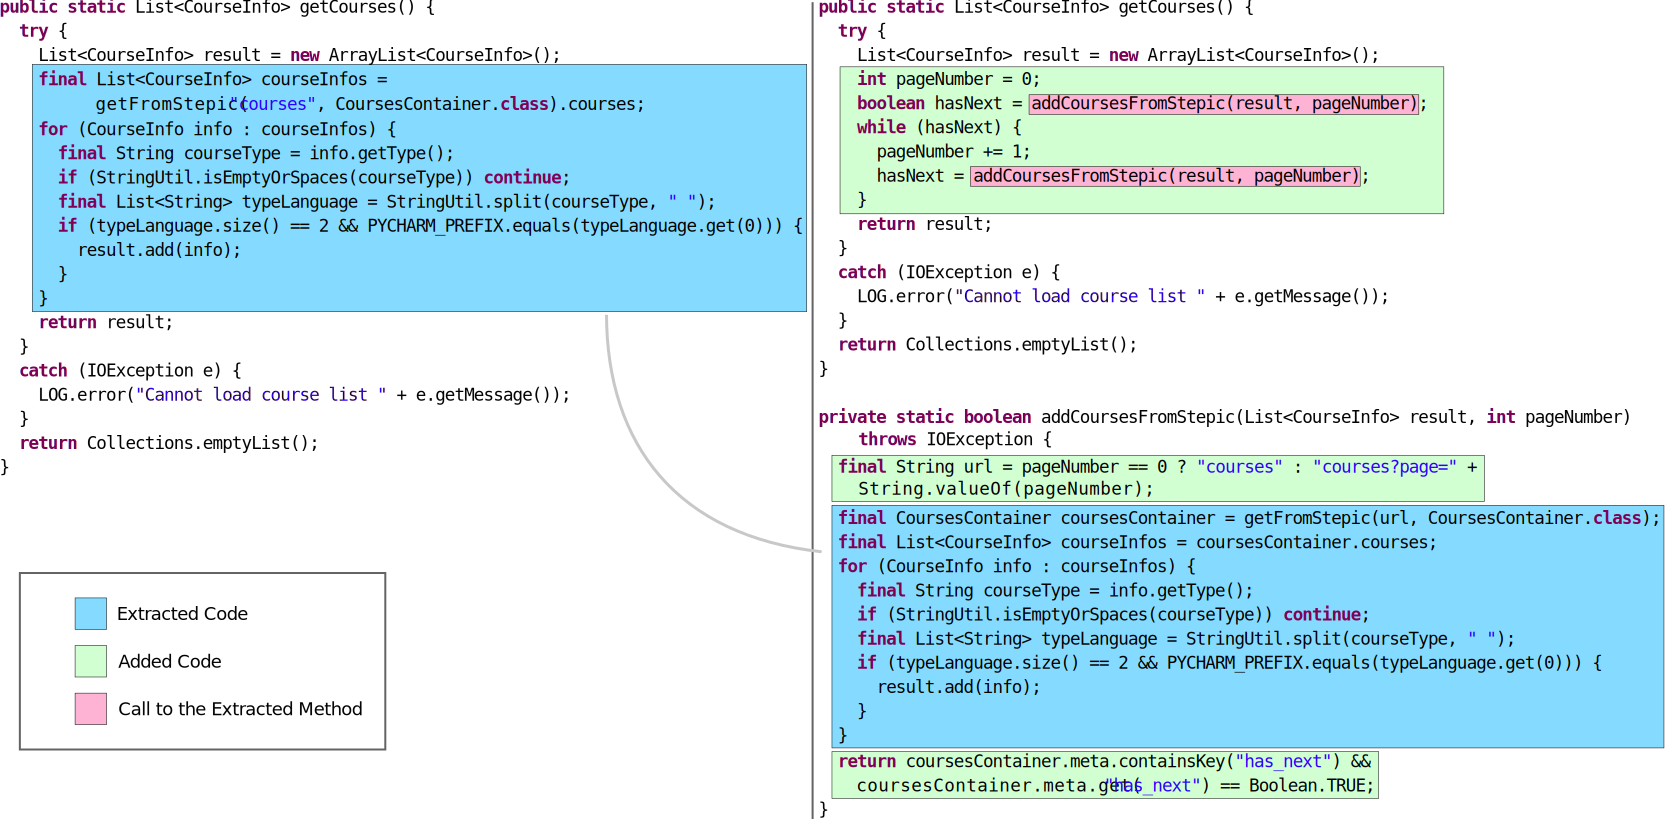
\includegraphics[width=0.9\linewidth]{img/code-sample.pdf}
	\caption{Example of Extract Method refactoring that was required to reach a consensus.}
	\label{fig:consenus_example}
\end{figure}

By inspecting the source code changes, we can see that a part of the original method \texttt{getCourses()} (left-hand side of Figure~\ref{fig:consenus_example})
was extracted into method \texttt{addCoursesFromStepic()} (right-hand side of Figure~\ref{fig:consenus_example}).
After the refactoring, the extracted method is called twice, once before the \texttt{while} loop added in the original method, and once inside the \texttt{while} loop.
For this reason, Author\#1 labeled this case as ``Avoid duplication'', since the extracted method is reused two times after the refactoring.
However, the extracted method contains additional new code to compute properly the URL based on the page number passed as a parameter (first line in the extracted method),
and to return a \texttt{boolean} indicating if there exists a next page (last line in the extracted method).
For this reason, Author\#2 labeled this case as ``Facilitate extension'', since the extracted method also helps to implement the new pagination requirement.
After deliberation, the authors reached a consensus by keeping both theme labels, since the extracted method serves both purposes of reuse and extension.






\subsection{Examined Refactorings}

We monitored \totalProjects Java projects during the study period, and found commits in \activeProjects projects (\activeProjectsPercentage), i.e., 277 projects remained inactive.
We also found \refactoredProjects projects with refactoring activity, as detected by \toolName (including false positives).
In these projects, \detectedRefactorings refactoring instances were detected (in \commitsWithDetectedRefactoring commits), and were manually inspected by the first author of the study to confirm whether they are indeed true positives.
 
\begin{table}[ht]
\centering
\renewcommand{\arraystretch}{1.2}
\caption{Refactoring activity}
\label{TabRefactoringActivity}
\begin{tabular}{@{}l@{\hskip 6pt}r@{\hskip 6pt}r@{\hskip 6pt}rr@{\hskip 6pt}r@{}} \toprule
Refactoring & TP & FP & Prec. & Com. & Proj.\\ \midrule
{\textsc Extract Method} & 468 & 135 & 0.78 & 312 & 136 \\
{\textsc Move Class} & 432 & 512 & 0.46 & 85 & 60 \\
{\textsc Move Attribute} & 129 & 44 & 0.75 & 45 & 38 \\
{\textsc Rename Package} & 105 & 0 & 1.00 & 25 & 24 \\
{\textsc Move Method} & 99 & 48 & 0.67 & 40 & 31 \\
{\textsc Inline Method} & 58 & 67 & 0.46 & 44 & 36 \\
{\textsc Pull Up Method} & 33 & 1 & 0.97 & 18 & 17 \\
{\textsc Pull Up Attribute} & 23 & 1 & 0.96 & 11 & 11 \\
{\textsc Extract Superclass} & 22 & 11 & 0.67 & 18 & 16 \\
{\textsc Push Down Method} & 16 & 1 & 0.94 & 6 & 6 \\
{\textsc Push Down Attribute} & 15 & 1 & 0.94 & 7 & 7 \\
{\textsc Extract Interface} & 11 & 8 & 0.58 & 10 & 9 \\
\midrule
Total & 1411 & 830 & 0.63 & 539 & 185 \\
\bottomrule \end{tabular}
\end{table}

Table~\ref{TabRefactoringActivity} shows the number of true positives (TP), false positives (FP), and precision (Prec.) of \toolName by refactoring type,
as computed after the manual inspection of the detected refactorings.
In general, our tool achieves very high precision for {\textsc Rename Package} (100\%), {\textsc Pull Up/Push Down Attribute/Method} refactorings (over 94\%),
and relatively high precision for {\textsc Extract Method} and {\textsc Move Attribute} refactorings (over 75\%),
while the precision for {\textsc Move Method} and {\textsc Extract Superclass} is 67\%.
However, for some refactorings the precision is closer to 50\%, namely {\textsc Extract Interface} (58\%), {\textsc Inline Method} (46\%),
and {\textsc Move Class} (46\%).
We observed several cases of inner classes falsely detected as moved, because their enclosing class was simply renamed.
By supporting the detection of {\textsc Rename Class} refactoring, we could improve {\textsc Move Class} precision.
It should be emphasized that we asked the developers only about the true positives detected by \toolName.
In comparison to the results presented in Section~\ref{sec:precision_recall}, the precision is lower,
because the commits analyzed from GitHub projects may include tangled changes, while the commits analyzed in Section~\ref{sec:precision_recall} include only refactoring operations.
Tangled changes make the detection of refactorings more challenging, thus resulting in more false positives.
Finally, Table~\ref{TabRefactoringActivity} shows the number of distinct commits (Com.) and projects (Proj.) 
containing at least one true positive refactoring
(\commitsWithTruePositiveRefactoring out of \commitsWithDetectedRefactoring commits and 185 out of \refactoredProjects projects with detected refactorings contain at least one true positive refactoring).

\begin{comment}
Table~\ref{TabRefactoringActivityProject} shows the top-10 projects in terms of number of commits 
containing refactorings (considering only true positives). This table also presents the number of 
different refactoring types detected in each project (last column).

\begin{table}[ht]
\centering
\renewcommand{\arraystretch}{1.2}
\caption{Refactoring activity by project}
\label{TabRefactoringActivityProject}
\begin{tabular}{@{}lrr@{}} \toprule
Project & Commits  & Ref. types\\ \midrule
{\textsc JetBrains/intellij-community} & 37 & 9 \\
{\textsc facebook/buck} & 17 & 6 \\
{\textsc apache/hive} & 15 & 3 \\
{\textsc neo4j/neo4j} & 15 & 7 \\
{\textsc apache/cassandra} & 14 & 4 \\
{\textsc gradle/gradle} & 13 & 9 \\
{\textsc VoltDB/voltdb} & 13 & 5 \\
{\textsc CyanogenMod/android_fra\ldots} & 11 & 4 \\
{\textsc hazelcast/hazelcast} & 10 & 7 \\
{\textsc SonarSource/sonarqube} & 10 & 6 \\
\bottomrule \end{tabular}
\end{table}
\end{comment}








\section{Why do Developers Refactor?}

\begin{table}[htb]
\centering
\renewcommand{\arraystretch}{1.2}
\caption{{\textsc Extract Method} motivations}
\label{TabExtractMethodMotivations}
\footnotesize 
\begin{tabular}{@{}p{4cm}p{8cm}r@{}} \toprule
Theme & Description & \multicolumn{1}{c@{}}{Occur.}\\ \midrule
Extract reusable method & Extract a piece of reusable code from a single place and call the extracted method in multiple places. &  \minibarn{43}{43} \\
Introduce alternative method signature & Introduce an alternative signature for an existing method (e.g., with additional or different parameters) and make the original method delegate to the extracted one. &  \minibarn{25}{43} \\
Decompose method to improve readability & Extract a piece of code having a distinct functionality into a separate method to make the original method easier to understand. &  \minibarn{21}{43} \\
Facilitate extension & Extract a piece of code in a new method to facilitate the implementation of a feature or bug fix, by adding extra code either in the extracted method, or in the original method. &  \minibarn{15}{43} \\
Remove duplication & Extract a piece of duplicated code from multiple places, and replace the duplicated code instances with calls to the extracted method. &  \minibarn{14}{43} \\
Replace Method preserving backward compatibility & Introduce a new method that replaces an existing one to improve its name or remove unused parameters. The original method is preserved for backward compatibility, it is marked as deprecated, and delegates to the extracted one. &  \minibarn{6}{43} \\
Improve testability & Extract a piece of code in a separate method to enable its unit testing in isolation from the rest of the original method. &  \minibarn{6}{43} \\
Enable overriding & Extract a piece of code in a separate method to enable subclasses override the extracted behavior with more specialized behavior. &  \minibarn{4}{43} \\
Enable recursion & Extract a piece of code to make it a recursive method. &  \minibarn{2}{43} \\
Introduce factory method & Extract a constructor call (class instance creation) into a separate method. &  \minibarn{1}{43} \\
Introduce async operation & Extract a piece of code in a separate method to make it execute in a thread. &  \minibarn{1}{43} \\
\bottomrule \end{tabular}

\end{table}

In this section, we present the results for the first question answered by the developers, regarding the reasons behind 
the application of the refactorings we detected. Based on the results of the thematic analysis process (Section~\ref{sec:study_design}), we compile a catalogue of \totalMotivationThemes distinct motivations.
We dedicate Section~\ref{SecExtractMethodMotivations} to discuss {\textsc Extract Method}, which is the most frequently 
occurring refactoring operation in our study, and also the one with the most observed motivations (11). 
Section~\ref{sec:other:motivations} presents the motivations for the remaining refactorings.
%Last, we discuss our main findings in Section~\ref{sec:discussion}. 


\subsection{Motivations for Extract Method}
\label{SecExtractMethodMotivations}
\begin{table}[htbp]
\centering
\renewcommand{\arraystretch}{1.2}
\caption{Motivations for {\textsc Move Class, Attribute, Method (MC, MA, MM)}, {\textsc Rename Package (RP)} {\textsc Inline Method (IM)}, {\textsc Extract Superclass, Interface (ES, EI)}, {\textsc Pull Up Method, Attribute (PUM, PUA)}, {\textsc Push Down Attribute, Method (PDA, PDM)} }
%\caption{Motivations for other refactoring types}
\label{TabOtherMotivations}
\footnotesize
\resizebox{\linewidth}{!}{
\begin{tabular}{@{}lp{5cm}p{12cm}r@{}} \toprule
Type & Theme & Description & \multicolumn{1}{c@{}}{Occur.}\\
\midrule
MC & Move class to appropriate container & Move a class to a package that is more functionally or conceptually relevant. & \minibarn{13}{15} \\
MC & Introduce sub-package & Move a group of related classes to a new subpackage. & \minibarn{7}{15} \\
MC & Convert to top-level container & Convert an inner class to a top-level class to broaden its scope. & \minibarn{4}{15} \\
MC & Remove inner classes from deprecated container & Move an inner class out of a class that is marked deprecated or is being removed. & \minibarn{3}{15} \\
MC & Remove from public API & Move a class from a package that contains external API to an internal package, avoiding its unnecessary public exposure. & \minibarn{2}{15} \\
MC & Convert to inner class & Convert a top-level class to an inner class to narrow its scope. & \minibarn{2}{15} \\
MC & Eliminate dependencies & Move a class to another package to eliminate undesired dependencies between modules. & \minibarn{1}{15} \\
MC & Eliminate redundant sub-package & Eliminate a redundant nesting level in the package structure. & \minibarn{1}{15} \\
MC & Backward compatibility & Move a class back to its original package to maintain backward compatibility. & \minibarn{1}{15} \\
\midrule
MA & Move attribute to appropriate class & Move an attribute to a class that is more functionally or conceptually relevant. & \minibarn{15}{15} \\
MA & Remove duplication & Move similar attributes to another class where a single copy of them can be shared, eliminating the duplication. & \minibarn{4}{15} \\
\midrule
RP & Improve package name & Rename a package to better represent its purpose. & \minibarn{8}{15} \\
RP & Enforce naming consistency & Rename a package to conform to project's naming conventions. & \minibarn{3}{15} \\
RP & Move package to appropriate container & Move a package to a parent package that is more functionally or conceptually relevant. & \minibarn{2}{15} \\
\midrule
MM & Move method to appropriate class & Move a method to a class that is more functionally or conceptually relevant. & \minibarn{8}{15} \\
MM & Move method to enable reuse & Move a method to a class that permits its reuse by other classes. & \minibarn{3}{15} \\
MM & Eliminate dependencies & Move a method to eliminate dependencies between classes. & \minibarn{3}{15} \\
MM & Remove duplication & Move similar methods to another class where a single copy of them can be shared, eliminating duplication. & \minibarn{1}{15} \\
MM & Enable overriding & Move a method to permit subclasses to override it. & \minibarn{1}{15} \\
\midrule
IM & Eliminate unnecessary method & Inline and eliminate a method that is unnecessary or has become too trivial after code changes. & \minibarn{13}{15} \\
IM & Caller becomes trivial & Inline and eliminate a method because its caller method has become too trivial after code changes, so that it can absorb the logic of the inlined method without compromising readability. & \minibarn{2}{15} \\
IM & Improve readability & Inline a method because it is easier to understand the code without the method invocation. & \minibarn{1}{15} \\
\midrule
ES & Extract common state/behavior & Introduce a new superclass that contains common state or behavior from its subclasses. & \minibarn{7}{15} \\
ES & Eliminate dependencies & Introduce a new superclass that is decoupled from specific dependencies of a subclass. & \minibarn{1}{15} \\
ES & Decompose class & Extract a superclass from a class that holds many responsibilities. & \minibarn{1}{15} \\
\midrule
PUM & Move up common methods & Move common methods to superclass. & \minibarn{8}{15} \\
\midrule
PUA & Move up common attributes & Move common attributes to superclass. & \minibarn{7}{15} \\
\midrule
EI & Facilitate extension & Introduce an interface to enable different behavior. & \minibarn{1}{15} \\
EI & Enable dependency injection & Introduce an interface to facilitate the use of a dependency injection framework. & \minibarn{1}{15} \\
EI & Eliminate dependencies & Introduce an interface to avoid depending on an existing class/interface. & \minibarn{1}{15} \\
\midrule
PDA & Specialized implementation & Push down an attribute to allow specialization by subclasses. & \minibarn{2}{15} \\
PDA & Eliminate dependencies & Push down attribute to subclass so that the superclass does not depend on a specific type. & \minibarn{1}{15} \\
\midrule
PDM & Specialized implementation & Push down a method to allow specialization by subclasses. & \minibarn{1}{15} \\
\bottomrule \end{tabular}
}
\end{table}


Table~\ref{TabExtractMethodMotivations} describes 11 motivations for {\textsc Extract Method} refactoring and the number of occurrences for each of them. 
The most frequent motivation is to extract a reusable method (43 instances).
In this case, the refactoring is motivated by the immediate reuse of a piece of code
in multiple other places, in addition to the place from which it was originally extracted.
We often observe a concern among developers to reuse code wherever possible, by extracting pieces of reusable code.
This is illustrated by the following comments:\margin

\noindent{\em \quotes{These refactorings were made because of code reusability. I needed to use the same 
code in new method. I always try to reuse code, because when there's a lot of code redundancy it gets
overwhelmingly more complicated to work with the code in future, because when something change in code 
that has it's duplicate somewhere, it usually needs to be changed also there.}}\margin

%\noindent{\em [REPLACE BY NEW ONE] There was already code duplication, but the bug fix required a cut-and-paste, 
%which made it code triplication. That was above my pain level so I decided to group the replicated code.}\margin

\noindent{\em \quotes{The reason for me to do the refactoring was: Don't repeat yourself (DRY).}}\margin

%\noindent{\em The existing piece of code obtaining such annotation options from parameters
%of compilerArgument configuration can be reused for compilerArgs. So, this code was moved 
%to a separate method for reuse.}\margin


The second most frequent motivation is to introduce an alternative method signature for an existing method
 (25 instances), e.g.,~with extra parameters.
To achieve that, the body of the existing method is extracted to a 
new one with an updated signature and additional logic to handle the extended variability.
The original  method is changed to delegate to the new one, passing some default values for the new parameters.
The following comment illustrates this case:\margin

\noindent{\em \quotes{The extracted method \texttt{values(names List<String>, values List<Object>)} could be of 
help for some users using Lists instead of arrays, and because the implementation already transformed the provided 
arrays into Lists internally.}}\margin


Decomposing a method for improving readability (21 instances) is the third most frequent motivation. Typically, 
this corresponds to a {\em Long Method} code smell~\citep{Fowler:1999}, as illustrated in this comment:\margin

\noindent{\em \quotes{The method was so long that it didn't fit onto the screen anymore, so I moved out parts.}}\margin


The next two motivations are to facilitate extension (15 instances) and to remove duplication (14 instances).
In the first case, a method is decomposed to facilitate the implementation of a new feature or the fix of a bug by adding code either in the extracted or in the 
original method, as illustrated in this comment:\margin

\noindent{\em \quotes{I was fixing an exception, in order to do that I had to add the same 
	code to 2 different places. So I extracted initial code, replace 
	duplicate with the extracted method and add the `fix' to the extracted 
	method.}}\margin

In the second case (i.e., remove duplication), a piece of duplicated code is extracted from multiple places into a single method, as illustrated in the following comments:\margin

\noindent{\em \quotes{I refactored shared functionality into a single method.}}\margin

\noindent{\em \quotes{I checked how other test methods create testing User objects and noticed that it takes two lines of code that were repeated all over the test class.
	So I abstracted these two lines of code into a method for better readability and then reused the method in all the places that had the same code.}}\margin

Finally, two other important motivations are to improve testability (6 instances) and to replace a method by preserving backward compatibility (6 instances).
In the first case, the decomposition enables the developer to test parts 
of the code in isolation, as illustrated in this comment:\margin

\noindent{\em \quotes{I wanted to test the part of \texttt{authenticate()} which verifies that a member is element of a set, and that would have been more complex using \texttt{authenticate} directly.}}\margin

In the second case, the goal is to introduce a method having the same functionality with an already existing one, but a different signature (e.g., improved name, or removed unused parameter), and at the same time preserve the public API by making the original method delegate to the new one.
This motivation is best illustrated in the following comment:\margin

\noindent{\em \quotes{I did that refactoring because essentially I wanted to rename the
	functions involved - you'll see the old functions just forward straight to
	the new ones. But I didn't just rename because other code in other projects
	might be referring to the old functions, so they would need to still be
	present (I guess they should have been marked as @deprecated then, but I
	was a bit lazy here).}}
%Table~\ref{TabExtractMethodMotivations} also presents the less frequent motivations: \textbf{Enable overrides}, 
%\textbf{Enable recursion}, \textbf{Introduce factory method} and \textbf{Introduce async operation}.





\subsection{Motivations for Other Refactorings}
\label{sec:other:motivations}


Table~\ref{TabOtherMotivations} presents the motivations for the remaining refactorings.
We found nine different motivations for {\textsc Move Class}.
The two most frequent motivations are to move a class to a package that is more functionally or conceptually related to 
the purpose of the class (13 instances), and to introduce a sub-package (7 instances). The first one is illustrated by the following comment:\margin

%\noindent{\em I have moved CompositeCodecTests to the
%org.springframework.integration.codec.kryo package because that class
%contains functionality exactly about the Kryo (PojoCodec).}\margin

\noindent{\em \quotes{This refactoring was done because common interface for those classes 
lived in \texttt{org.neo4j.kernel.impl.store.\\record}, while most of it's implementors lived in 
\texttt{org.neo4j.\\kernel.impl.store} which did not make sense because all of them are actually records.}}\margin

%The third more frequent motivation is introduce a sub-package, as in the example below:\margin

%\noindent{\em \quotes{The functionality of that class was enhanced. For that, it needed 
%several more algorithms for mapping data (\ldots).
%As the 2 new mapping classes are only relevant to the one class existing before 
%the refactoring, it made sense to move all 3 into a sub package.}}\margin


For {\textsc Move Attribute}, the most common motivation is also to move the attribute to an 
appropriate class that is more functionally or conceptually relevant (15 instances), as in the 
example below:\margin

\noindent{\em \quotes{In this case, each of these fields was moved as their relevance changed. As
\texttt{UserService} already handles the login process, it makes sense that changes
to the login process should be encapsulated within \texttt{UserService}.}}\margin

Remove duplication is another motivation for moving an attribute, as illustrated by the following 
comment:\margin

\noindent{\em \quotes{The attributes were duplicated, so I moved them to the proper common place.}}\margin


For {\textsc Rename Package}, the most common motivation is to update the name of a package to better represent its purpose (8 instances), as in the example below:\margin

\noindent{\em \quotes{This was a simple package rename. \texttt{test} seems to fit better than \texttt{tests} here as a single test can be executed too.}}\margin

We found three main reasons for a {\textsc Move Method} refactoring: move a method to an appropriate 
class (8 instances), move a method to enable reuse (3 instances), and move a method to eliminate 
dependencies (3 instances). 
%\noindent{\em \quotes{Move \texttt{timestampStatsOfIndex()} into \texttt{EsIndexRangeService} to resolve circular dependency.}}\margin
The most frequent motivation for {\textsc Inline Method} is to eliminate 
an unnecessary or trivial method, as illustrated in the comment:\margin

\noindent{\em \quotes{Since the method was a one-liner and was used only in one place, inlining it didn't make 
the code more complex. On the other hand, it allowed to lessen calls to \texttt{getVirtualFile()}.}}\margin

{\textsc Extract Superclass} is usually applied to introduce a new class with state or behavior that can be
shared by subclasses (7 instances).
{\textsc Pull Up Method/Attribute} is performed to move common code to an existing superclass (8 and 7 instances, 
respectively). {\textsc Extract Interface} and {\textsc Push Down Attribute/Method} are 
less popular refactorings and thus their motivations have at most two instances.












\section{Refactoring Automation}
\label{SecAutomatedRefactoring}

In this section, we discuss the results drawn from the second question answered by the developers, regarding the 
use (or not) of automatic refactoring tools provided by their IDEs to apply the refactorings we presented. 
First, in Section~\ref{SecRefactoringToolsUnderused}, we present how many of the interviewed developers applied the
refactoring(s) automatically. We also present which refactoring types are more frequently applied with tool support.
In Section~\ref{SecReasonForManualRefactoring}, we discuss some insights drawn from developers' answers that explain
why refactoring is still applied manually in most of the cases.
Last, in Section~\ref{SecIde}, we present additional details regarding which IDE developers most often used
for refactoring.



\subsection{Are refactoring tools underused?}
\label{SecRefactoringToolsUnderused}

% Discarding Not answered, we have 174 in total
Table~\ref{TabManualVsAutomated} shows the results for this question.
95 developers (55\% of valid answers) answered that the refactoring was performed manually without tool support;
66 developers (38\%) answered that the refactoring engine of an IDE was used;
13 developers (7\%) answered that the refactoring was partially automated. 
In summary, refactoring is probably more often applied manually than with refactoring tools.

\begin{table}[htbp]
\centering
\renewcommand{\arraystretch}{1.2}
\caption{Manual vs. automated refactoring}
\label{TabManualVsAutomated}
\begin{tabular}{@{}lr@{}} \toprule
Modification & \multicolumn{1}{c@{}}{Occurrences} \\ \midrule
Manual & \minibarn{95}{95} \\
Automated & \minibarn{66}{95} \\
Not answered & \minibarn{48}{95} \\
Partially automated & \minibarn{13}{95} \\
\bottomrule \end{tabular}
\end{table}


We also counted the percentage of automated refactorings by refactoring type, as presented in Table~\ref{TabRefactoringTypeAutomated}.
{\textsc Rename Package} is the refactoring most often performed with tool support (58\%), followed by {\textsc Move Class} (50\%).
%{\textsc Move Class} is the refactoring most often performed with tool support (48\%). %, followed by {\textsc Push Down Attribute} (33\%).
Three other refactorings are performed automatically in around a quarter of the cases: {\textsc Extract Method} (29\%), {\textsc Move Method} (26\%), and {\textsc Move Attribute} (24\%).
{\textsc Inline Method} follows with 18\% of automatic applications.
Finally, for the remaining refactorings, we do not have a large number of instances to draw safe conclusions (maximum 9 instances),
but there is a consistent trend showing that inheritance-related refactorings are mostly manually applied.
%The other six refactorings types are performed at most 18\% of the cases with the support of a tool.  

\begin{table}[htbp]
\centering
\renewcommand{\arraystretch}{1.2}
\caption{Refactoring automation by type}
\label{TabRefactoringTypeAutomated}
\begin{tabular}{@{}lrr@{}} \toprule
Refactoring Type & \multicolumn{1}{c}{Occurrences} & \multicolumn{1}{c@{}}{Automated \%} \\ \midrule
{\textsc Extract Method} & \minibarn{118}{118} & \minibard{29}{100} \\
{\textsc Move Class} & \minibarn{36}{118} & \minibard{50}{100} \\
{\textsc Move Attribute} & \minibarn{21}{118} & \minibard{24}{100} \\
{\textsc Move Method} & \minibarn{19}{118} & \minibard{26}{100} \\
{\textsc Inline Method} & \minibarn{17}{118} & \minibard{18}{100} \\
{\textsc Rename Package} & \minibarn{12}{118} & \minibard{58}{100} \\
{\textsc Extract Superclass} & \minibarn{9}{118} & \minibard{11}{100} \\
{\textsc Pull Up Method} & \minibarn{9}{118} & \minibard{11}{100} \\
{\textsc Pull Up Attribute} & \minibarn{7}{118} & \minibard{14}{100} \\
{\textsc Extract Interface} & \minibarn{3}{118} & \minibard{0}{100} \\
{\textsc Push Down Attribute} & \minibarn{3}{118} & \minibard{33}{100} \\
{\textsc Push Down Method} & \minibarn{2}{118} & \minibard{0}{100} \\
\bottomrule \end{tabular}
\end{table}



\subsection{Why do developers refactor manually?}
\label{SecReasonForManualRefactoring}

29 developers explained in their answers why they did not use a refactoring tool. 
Table~\ref{TabManualRefactoringReasons} shows five distinct themes we identified in these answers.

\begin{table}[htbp]
\centering
\renewcommand{\arraystretch}{1.2}
\caption{Reasons for not using refactoring tools}
\label{TabManualRefactoringReasons}
\footnotesize
\begin{tabular}{@{}p{0.74\linewidth}r@{}} \toprule
Description & \multicolumn{1}{c@{}}{Occurrences}\\ \midrule
The developer does not trust automated support for complex refactorings. & \minibarn{10}{10} \\
Automated refactoring is unnecessary, because the refactoring is trivial and can be manually applied. & \minibarn{8}{10} \\
The required modification is not supported by the IDE. & \minibarn{6}{10} \\
The developer is not familiar with the refactoring capabilities of his/her IDE. & \minibarn{3}{10} \\
%The developer did not consider using refactoring tools, but admitted he/she should have done so. 
The developer did not realize at the moment of the refactoring that he/she could have used refactoring tools.
& \minibarn{2}{10} \\
\bottomrule \end{tabular}
\end{table}

Lack of trust (10 instances) was the most frequent reason. Some developers do not trust
refactoring tools for complex operations that involve code manipulation and only use them for renaming
or moving:\margin

\noindent{\em \quotes{I don't trust the IDE for things like this, and usually lose other comments, notation, 
spacing from adjacent areas.}}\margin

\noindent{\em \quotes{I'd say developers are reluctant to let a tool perform anything but trivial refactorings, 
such as the ones you picked up on my commit.}}\margin

On the other hand, some developers also think that tool support is unnecessary in simple cases (8 instances).
Sometimes the operation may involve only local changes and is trivial to do by hand. Thus, calling a 
special operation to do it is considered unnecessary, as illustrated by this comment:\margin

\noindent{\em \quotes{Automated refactoring is overkill for moving some private fields.}}\margin

Additionally, developers also mentioned: lack of tool support for the specific refactoring they were 
doing (6 instances), not being familiar with refactoring features of the IDE (3~instances), and not
realizing they could use refactoring tools at the moment of the refactoring (2~instances).



\subsection{What IDEs developers use for refactoring?}
\label{SecIde}

When answering to our emails, 83 developers spon\-ta\-ne\-ously mentioned which IDE they use. 
Therefore, we decided to investigate these answers, specially because our study is not dependent
on any IDE, and thus differs from previous studies which are usually based only on 
Eclipse data~\citep{MurphyHill2012,negara2013}.
Table~\ref{TabIdePopularity} shows the most common IDEs mentioned in these answers and the percentage 
of refactorings performed automatically in these cases.
139 developers (63\%) did not explicitly mention an IDE when answering this question. 
Considering the answers citing an IDE, IntelliJ IDEA is the most popular one. 
It also has the highest ratio of refactorings performed automatically (71\%). 
Since 11 {\textsc JetBrains/\-intellij-community} (and related plug-ins) developers answered to our questions, 
we also investigated the answers separately in two groups, namely 
%Table~\ref{TabIntellijDevelopers} breaks the IntelliJ IDEA answers in two gropus: 
answers from IntelliJ IDEA developers and from IntelliJ IDEA users.
We observed that the ratio of automated refactorings in both groups is very similar (73\% vs. 70\%).
Therefore, the responses from these 11 IntelliJ IDEA developers do not bias the percentage of automated refactoring reported for 
IntelliJ IDEA. 



\begin{table}[htbp]
\centering
\renewcommand{\arraystretch}{1.2}
\caption{IDE popularity}
\label{TabIdePopularity}
\begin{tabular}{@{}lrr@{}} \toprule
IDE & \multicolumn{1}{c}{Occurrences} & \multicolumn{1}{c@{}}{Automated \%} \\ \midrule
Editor not mentioned & \minibarn{139}{139} & \minibard{12}{100} \\
IntelliJ IDEA & \minibarn{51}{139} & \minibard{71}{100} \\
Eclipse & \minibarn{18}{139} & \minibard{44}{100} \\
NetBeans & \minibarn{8}{139} & \minibard{50}{100} \\
Android Studio & \minibarn{4}{139} & \minibard{25}{100} \\
Text Editor & \minibarn{2}{139} & \minibard{0}{100} \\
\bottomrule \end{tabular}
\end{table}





\section{Discussion}

In this section, we discuss the main findings of our study.\margin

%\noindent\textbf{Detecting Refactorings:}\\


\noindent\textbf{Refactoring Motivations:} Our study confirms that {\textsc Extract Method} is  the 
``Swiss army knife of refactorings''~\citep{tsantalis_empiricalstudy}. It is the refactoring with the most motivations (11 in total).
In comparison to the study of ~\cite{tsantalis_empiricalstudy}, there is an overlap in the reported motivation themes for {\textsc Extract Method}.
We found some new themes, such as \emph{improve testability} and \emph{enable recursion}, but we did not find any instances of
the themes \emph{encapsulate field} and \emph{hide message chain}, reported by~\cite{tsantalis_empiricalstudy}, which are related to code smell resolution.
We assume these different themes are due to the nature of the examined projects, since~\cite{tsantalis_empiricalstudy} examined only
three libraries and frameworks, while in this study we examined \studiedProjects projects from various domains including standalone applications.
By comparing to the code symptoms that initiate refactoring reported in the study by \cite{kim-tse-2014}, we found the \emph{readability},
\emph{reuse}, \emph{testability}, \emph{duplication}, and \emph{dependency} motivation themes in common.
%Most of these motivations are related to enabling conditions to complete a maintenance task.

Most of the refactoring motivations we found have the intention to facilitate or even enable the completion of the maintenance task that the developer is working on.
For instance, \emph{extract reusable method}, \emph{introduce alternative method signature}, and \emph{facilitate extension}
are among the most frequent motivations, and all of them involve enhancing the functionality of the system.
Therefore, {\textsc Extract Method} is a key operation to complete other
maintenance tasks, such as adding a feature or fixing a bug.
In contrast, only two out of the 11 motivations we found (\emph{decompose method to improve readability} and \emph{remove duplication}) are targeting code smells. % 35/138 = 25\% os total instances
This finding could motivate researchers and tool builders to design
refactoring recommendation systems~\citep{Tsantalis:2011, Silva:2014, Tairas:2012, Hotta:2012, Meng:2015, Tsantalis:2015}
that do not focus solely on detecting refactoring opportunities for the sake of code smell resolution, but can support other refactoring motivations as well.
%Currently, most of these tools detect refactoring opportunities as a means to resolve detected code smells.

We also observe that developers are seriously concerned about avoiding code duplication, when working on a given maintenance task. They often use refactorings---especially {\textsc Extract Method}---to
achieve this goal, as illustrated by the following comments:\margin

\noindent{\em \quotes{I need to add a check to both the then- and the else-part of an if-statement. 
This resulted in more duplicated code than I was comfortable with.}}\margin

\noindent{\em \quotes{There was already code duplication, but the bug fix required another cut-and-paste, 
which made it code triplication. That was above my pain level so I decided to group the replicated code 
out into \texttt{bail()}.}}\margin

The other refactorings we analyzed are typically performed to improve the system design. For example,
the most common motivation for {\textsc Move Class}, {\textsc Move Attribute}, and {\textsc Move Method} is to reorganize
code elements, so that they have a stronger functional or conceptual relevance.\margin


\begin{comment}

%, there are many existing refactoring recommendation approaches based solely in  code smells~\citep{Tsantalis:2011, Silva:2014, Tairas:2012, Hotta:2012, Meng:2015, Tsantalis:2015}, but none that is centered in facilitating code evolution.  Thus, researchers may investigate new approaches that explore this gap.

%In light of the results we presented, we argue that facilitating the evolution of the system is a  stronger driver for refactoring effort than fixing existing code smells. In fact, when we look at {\textsc Extract Method}, most of the refactoring motivations we found have the intention to facilitate the maintenance task that the developer is currently working on. For instance, \emph{extract reusable method} and \emph{introduce alternative method signature} are the most frequent motivations, and both of them involve adding code to the system. Besides, only two of the 11 motivations (decompose method to improve readability and remove duplication) are code smells centered. % 35/138 = 25\% os total instances However, there are many existing refactoring recommendation approaches based solely in  code smells~\citep{Tsantalis:2011, Silva:2014, Tairas:2012, Hotta:2012, Meng:2015, Tsantalis:2015}, but none that is centered in facilitating code evolution. Thus, researchers may investigate new approaches that explore this gap. \danilo{maybe give an example, but how?}
% Example

Among code smells, we should mention \emph{long method}, \emph{duplicated code}, and \emph{feature envy}
as important drivers for refactoring.
 %that code duplication is an issue that developers do not tolerate.
It is interesting to observe developers not only removed duplication using 
{\textsc Extract Method}, {\textsc Move Attribute} and {\textsc Move Method}, but also tried to reuse code as 
much as possible, avoiding new duplicated code.
The little tolerance with code duplication became clear in comments such as:\margin


\noindent{\em \quotes{I need to add a check to both the then- and the else-part of an if-statement. 
This resulted in more duplicated code than I was comfortable with.}}\margin

\noindent{\em \quotes{There was already code duplication, but the bug fix required another cut-and-paste, 
which made it code triplication. That was above my pain level so I decided to group the replicated code 
out into bail().}}\margin


\end{comment}


%Thus, approaches that assist clone detection~\citep{Tairas:2012, Tsantalis:2015} may be improved to work in code 


\noindent\textbf{Automated vs. Manual Refactoring:} In a field study with Eclipse users, 
\cite{negara2013} report that most refactorings (52\%) are manually performed.
In our study, involving developers using a wider variety of IDEs, we found that 55\% of refactorings are manually performed. 
However, we also found that IntelliJ IDEA users tend to use more the refactoring tool support than other IDE users.
Moreover, the results for automated {\textsc Extract Method} refactorings are very similar in both studies: 28\% in our study vs. 30\% in their study.
While the total percentages of manually performed refactorings are very similar, we should
keep in mind that Negara et al.~counted simple refactorings, like renamings, which are more often applied with tool support.
%This difference is specially significant because they counted simple refactorings, like renamings. 
%However, the results for {\textsc Extract Method} are very similar in both studies: 28\% in our study, 
%against 30\% in theirs.
Compared to the study by \cite{MurphyHill2012},
where they report that 89\% of refactorings are performed manually (considering also renamings),
we detected significantly more automated refactorings.
%It's reasonable to assume that Automated refactoring tools have become more popular
We suspect this difference may be due to two reasons.
First, automated refactoring tools may have become more popular and reliable
over the last years. Second, our study involves developers using a broader range of IDEs, which may also 
influence how developers use refactoring tool support.

Regarding the reasons for not using automated refactoring, our results are in line with the three main factors found in the study by \cite{MurphyHill2012}: \emph{awareness}, \emph{opportunity}, and \emph{trust}. 
The exception is the argument that tool support is unnecessary in simple cases, which is not closely 
related to any of the three aforementioned factors.
However, the same argument can be observed in the study by \cite{kim-tse-2014}, in which some 
developers mention that they do not feel a great need for automated refactoring tools.\margin

\noindent\textbf{Refactoring Popularity:}
In this study we detected refactorings in \refactoredProjects 
of the monitored repositories in a time window of 61 days. Given that only \activeProjects out of the \totalProjects monitored 
repositories were active during that period, we found refactoring activity in 60.5\% of the repositories with at least
one commit. This shows that refactoring is a common practice, especially considering that 
frequent refactorings such as {\textsc Rename Class/Method/Field} were not considered.
\begin{comment}
It is also worth noting that only in 22\% of the commits containing refactoring the
developer mentioned it in the commit description. Thus, relying in such criterion to find refactorings 
would have been a serious limitation, as also suggested by the study of \cite{MurphyHill2012}.
\end{comment}

The top-5 most popular refactorings detected in our study are 
{\textsc Extract Method}, {\textsc Move Class}, {\textsc Move Attribute}, {\textsc Rename Package}, and {\textsc Move Method}.
%Moreover, {\textsc Move Class} refactorings normally occur in batch, as a result of renaming a package.
{\textsc Move Method} is the third most popular refactoring in the study by \cite{negara2013}.
The top-2 refactorings in this study ({\textsc Rename Local Variable} and {\textsc Extract Local Variable}) are low-level refactorings, which have not been considered in our study.
We focused on high-level refactorings, because they can be motivated by multiple factors.

Using a sample of 40 commits with manual and automated refactorings, \cite{MurphyHill2012} report that the two most popular refactorings are {\textsc Rename Constant} and {\textsc Push Down}. 
However, {\textsc Push Down} refactorings are among the least popular ones in our study. This difference 
may be related to the number of commits analyzed in the studies (40 vs. \commitsWithTruePositiveRefactoring commits in our study),
and the specialized nature of the software (i.e., the Eclipse IDE) examined by \cite{MurphyHill2012}.
%\nikos{This is not our most important finding. I moved it at the end.}




\section{Threats to Validity}

\noindent \textbf{External Validity}: This study is restricted to open source, Java-based, GitHub-hosted projects. Thus, 
we cannot claim that our findings apply to industrial systems, or to systems implemented in other programming languages.
However, we collected responses from \studiedDevelopers developers contributing in \studiedProjects different projects, which is one of the largest samples
of systems used in refactoring studies.\margin

\noindent \textbf{Internal Validity}: First, we use in the study a tool that detects refactorings by comparing 
two revisions of the code.
We evaluated the recall of this tool using a sample of 120 documented refactoring operations. We achieved a recall of 0.93.
However, we cannot guarantee a similar recall in the studied GitHub projects, because some commits might contain tangled changes making more difficult to isolate (or untangle \citep{Dias:2015}) the changes related to refactorings.
In addition, it is known that this kind of detection approach may miss refactorings that do not reach the 
version control system (e.g., sequences of overlapping refactorings applied to the same piece of code).
We claim this threat should be tolerated in large scale studies, where we cannot assume that the developers would be willing to install an external monitoring tool in their IDEs~\citep{negara2013}.
Furthermore, as we showed in this study, developers nowadays use IDEs from multiple vendors.
In order to cover as many IDEs as possible and strengthen the external validity,
a study based on monitoring would require to develop a separate version of this tool for each IDE.
Second, we cannot claim that the catalogue of motivations we propose is exhaustive.
Notably, we have a limited number of motivation themes 
for less frequent refactoring types, such as {\textsc Push Down Method/Attribute} and {\textsc Extract 
Interface}.
Third, to mitigate inconsistencies in the proposed themes, we rely on an initial classification
performed independently by two authors of the study, followed by a consensus building process.
We also make publicly available the responses collected from the developers and the proposed
refactoring motivation themes to provide a means for replication and verification.

\section{Conclusions}

In summary, the main conclusions and lessons learned are:

%\noindent{\textbf{Lessons learned:}}
\begin{enumerate}
	%\setlength\itemsep{0mm}
	\item Refactoring activity is mainly driven by changes in the requirements (i.e., new feature and bug fix requests)
	and much less by code smell resolution.
	Only 2 out of the 11 motivations for {\textsc Extract Method} were related to code smell resolution (\emph{remove duplication}, \emph{decompose method}) covering only 25\% (35/138) of the motivation instances.
	%Research on refactoring recommendation systems should refocus from code-smell-oriented to maintenance-task-oriented solutions.
	\item {\textsc Extract Method} is a key operation that serves multiple purposes, specially those related to code
	reuse and functionality extension. It is also used to improve the testability of code, and deprecate public API methods.
	%On the other hand, {\textsc Move Class}, {\textsc Move Attribute}, and {\textsc Move Method}
	%are mainly applied to reorganize code elements.
	\item The elimination of dependencies is the most common motivation among the \emph{move}/\emph{abstract} related refactorings.
	%({\textsc Move Class/Method}, {\textsc Extract Superclass/Interface})
	\item Manual refactoring is still prevalent (55\% of the developers refactored manually the code).
	In particular, inheritance related refactoring tool support seems to be the most under-used (only 10\% done automatically),
	while {\textsc Move Class} and {\textsc Rename Package} are the most trusted refactorings (over 50\% done automatically).
	\item The IDE plays an important role in the adoption of refactoring tool support. IntelliJ IDEA users perform more automated refactorings (71\% done automatically) than Eclipse users (44\%) and Netbeans users (50\%).
	\item Compared to the study by \cite{MurphyHill2012}, it seems that developers apply more automated refactorings nowadays.
	Our findings confirm \cite{negara2013} who collected data only from Eclipse IDE users, but our study covers developers using more IDEs.
	%\item Developers often apply refactorings manually, because they consider refactoring tool support unreliable or unnecessary. 
	%However, users of different IDEs behave differently (e.g.,~IntelliJ IDEA users rely more on refactoring tools).
\end{enumerate}

Based on our findings, we propose that future research on refactoring recommendation systems should refocus from 
code-smell-oriented to maintenance-task-oriented solutions.
This could be achieved by leveraging the recent advancements in feature location~\citep{Dit:2013} and requirements tracing to automatically locate the code
associated with a feature or bug fix request, or a requirement change, and recommend suitable refactorings that will make easier the completion
of the maintenance task.
We strongly believe this will boost the adoption of recommendation systems by the developers.
%Also, we encourage researchers to validate and extend the catalogue of motivations we compiled in future studies.




\begin{figure}[b]
	\centering
	\fbox{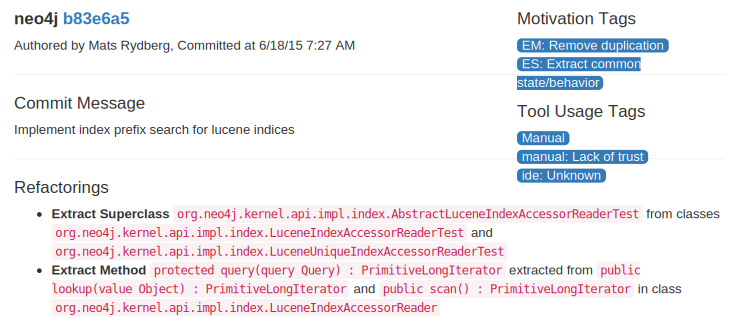
\includegraphics[width=0.96\linewidth]{img/screenshot.pdf}}
	\caption{An example of a commit with refactorings and their motivations.}
	\label{navDataset}
\end{figure}



\section{Artifact Description}

The data collected in this study is provided as an artifact, which is publicly available at:\margin

\noindent \url{http://aserg-ufmg.github.io/why-we-refactor}\margin

The dataset includes a list of 539 commits from 185 GitHub-hosted Java projects with 1,411 refactorings identified by the RefactoringMiner tool and confirmed with manual inspection. The detected refactorings cover 12 different types:
\begin{enumerate}
	%\setlength\itemsep{0mm}
	\item Extract Method (EM)
	\item Move Class (MC)
	\item Move Attribute (MA)
	\item Rename Package (RP)
	\item Move Method (MM)
	\item Inline Method (IM)
	\item Pull Up Method (UM)
	\item Pull Up Attribute (UA)
	\item Extract Superclass (ES)
	\item Push Down Method (DM)
	\item Push Down Attribute (DA)
	\item Extract Interface (EI)
\end{enumerate}


Additionally, the dataset includes a list of 222 commits with 463 refactorings and their motivations.
This is the subset of the commits with refactorings where the developers answered to our mails, describing the reasons for performing the detected refactorings. The motivation theme for each refactoring was proposed after analyzing all developers' answers using thematic-analysis. The dataset contains details of the themes assigned by each one of the two authors that independently analyzed each commit, and also the final themes derived after a discussion phase to reach a consensus.
Moreover, the dataset also includes information about the IDE used to perform the refactorings (if reported by the developer). In case the refactoring is performed manually, we also include a possible reason for not using the IDE refactoring tool support.


Figure~\ref{navDataset} illustrates one of these commits. 
In this example, there are two refactorings applied in the {\textsc neo4j} project. The first one is an {\textsc Extract Superclass}, in which the superclass \texttt{AbstractLuceneIndexAccessorReaderTest} was extracted from two other classes. This refactoring was performed to \emph{Extract common state/behavior}. The second refactoring, in which the method \texttt{query} was extracted from two other methods of class \texttt{LuceneIndexAccessorReader}, was performed to \emph{Remove duplication}. Additionally, the refactoring was performed manually (\emph{Manual} tag) due to a \emph{Lack of trust} in refactoring tools. Finally, the IDE is \emph{Unknown}, because it was not reported by the developer.
The dataset also includes meta-data about the commits (SHA1 hash, author, date, and time).


The dataset is available as a navigable web site, where researchers and practitioners can view and explore each commit including a refactoring with the motivation inferred in our study. However, we also provide the dataset in JSON format, to facilitate its import and use by other tools.

\subsection{License}

\noindent The dataset is distributed under the terms of the Creative Commons Attribution License, which permits unrestricted use, distribution, reproduction and adaptation in any me\-di\-um
%and for any purpose
provided that it is properly attributed.\\

\noindent{Danilo Silva, Nikolaos Tsantalis, Marco Tulio Valente. Why We Refactor? Confessions of GitHub Contributors. In \textit{Proceedings of the 24th International Symposium on the Foundations of Software Engineering} (FSE), 2016.}


\subsection{How to contribute}

Researchers are welcome to contribute to this dataset either reporting issues or submitting new data from different projects or commits. Such contributions should be made via GitHub \emph{issues} or \emph{pull requests} in the following repository:\margin

\noindent \url{https://github.com/aserg-ufmg/why-we-refactor}\margin




\input{theses-ch4.tex}
\chapter{Practical Applications of Refactoring Detection}
\label{ChPracticalApplications}

Throughout this thesis we discussed tools to mine refactorings from version histories and empirical studies that benefit from such techniques. In this chapter we discuss three practical applications of such tools.
We do not intend to thoroughly discuss all possible applications, but rather to exemplify that some relevant problems faced by development teams can be tackled with the help of such tools.
Particularly, RefDiff's multi-language design is an important advantage for the practical applications described below, as software projects are developed using different programming languages.


\section{Refactoring-aware Diff}
\label{SecRefactoringDiff}


One of the challenges developers face when refactoring, as reported in an in-depth study by \cite{kim-tse-2014}, is the difficulty of reviewing code after refactoring.
This is illustrated by the following comment from one of the developers interviewed by Kim~et~al.:\margin

\noindent{\em \quotes{It (refactoring) typically increases the number of lines/files involved in a check-in. That burdens code reviewers and
increases the odds that your change will collide with someone
else's change.}}\margin

In fact, version control systems are usually sensitive to rename and move refactoring,
which makes it hard for developers to understand code changes in some scenarios. 
As a concrete example, consider the code changes presented in Figure~\ref{FigRwDiff1}, which are taken from the \url{intellij-community} repository. In this figure, we present the code diff between two changed files. In the first one, \texttt{RunContentManagerImpl.java}, a large code block was removed, whilst in the second file (\texttt{ExecutionUtil.java}) a large code block was added. With a thoroughly analysis, we can note the the code removed from \texttt{RunContentManagerImpl.java} was actually moved to \texttt{ExecutionUtil.java}, i.e, the method \texttt{getLiveIndicator} was moved.
However this is not immediately obvious to a developer reviewing these changes, specially considering that there might be many other changed files in the commit. Moreover, although one can identify with some effort that the method \texttt{getLiveIndicator} has been moved, it will be much more difficult to identify small changes made to its body in this visualization.

%intellij-community ce5f9ff
\begin{figure}[htbp]
\centering
\includegraphics[width=\linewidth]{img/c1.png}
\caption{Typical diff visualization of a code change containing a moved method}
\label{FigRwDiff1}
\end{figure}


In contrast, consider the diff visualization presented in Figure~\ref{FigRwDiff2}. In this case, the diff is focused in the method that was moved, \texttt{getLiveIndicator}, before and after the change. We can clearly see that some changes have been made to the body of \texttt{getLiveIndicator}. Specifically, the annotations \texttt{@Nullable} and \texttt{@SuppressWarnings} were introduced, a new local variable \texttt{iSize} was declared, and the expression passed as the first argument to the \texttt{Ellipse2D.Double} constructor was changed.
All these changes are very hard to note in a traditional diff visualization, such as the one from Figure~\ref{FigRwDiff1}, but are easily discernible when we present the moved method compared with its counterpart.
Other refactoring types might benefit from such idea as well.
As a second example, it would also be convenient to highlight the differences between an extracted method and its originating code. This way, it would become easier to identify new statements added.
A similar reasoning can be applied to Move Class, Inline Method, and other refactoring types.

\begin{figure}[htbp]
\centering
\includegraphics[width=\linewidth]{img/c2.png}
\caption{Diff visualization focused on the moved method}
\label{FigRwDiff2}
\end{figure}

Thus, we can improve diff visualization using the information about the refactorings applied in a commit.
We expect that such refactoring-aware diff visualization solution would improve developers' ability to discern and understand code changes in the presence of refactorings, enabling them to concentrate on changes of behavior rather than on code modifications resulting from refactorings.


\section{Tracking changes of a code element}
\label{SecAppTrackChanges}

Although refactoring is very important to maintain a software system, it can make it harder to track code changes in the history, specially in the method/function level.
% https://github.com/facebook/react/commit/63aa7259b9f48886af545afcc06c29acf225b05f
For example, consider the \texttt{getReactRootElementInContainer} function from React project, depicted in Figure~\ref{FigGitBlameReact}.
\begin{figure}[htbp]
\centering
\includegraphics[width=\linewidth]{img/git-blame-react.png}
\caption{\textit{git-blame} visualization of the \texttt{ReactMount.js} file from React project, showing that function \texttt{getReactRootElementInContainer} was last modified by Mert Kahyao\u{g}lu}
\label{FigGitBlameReact}
\end{figure}
Suppose one is investigating the history of that function to find out who introduced the conditional statement in lines 85--89. Developers typically use the \textit{git-blame} tool for such tasks, as it shows what revision and author last modified each line of code of a file. However, although the \textit{git-blame} output shows that Mert Kahyao\u{g}lu was the last developer that modified the lines of code within \texttt{getReactRootElementInContainer}, this information may mislead one to think that he is the author of the function.
In fact, a deeper analysis of the history reveals that Mert Kahyao\u{g}lu actually moved the function from file \texttt{getReactRootElementInContainer.js} to \texttt{ReactMount.js}.
Thus, to find the actual author of those lines of code, one should inspect the history of changes of the original file of the function. Figure~\ref{FigGitBlameReactActualAuthor} shows that the conditional in lines 85--89 was actually introduced by Andrey Popp.


\begin{figure}[htbp]
\centering
\includegraphics[width=\linewidth]{img/git-blame-react-actual-author.png}
\caption{Diff visualization of the commit in witch the conditional inside function \texttt{getReactRootElementInContainer} was introduced, showing that the actual author is Andrey Popp}
\label{FigGitBlameReactActualAuthor}
\end{figure}

In summary, in the example above, the \textit{Move Function} refactoring split the history of \texttt{getReactRootElementInContainer}, making it harder to trace back the author of each line of code.
The frequency in which such situations occur makes this problem even more important. \cite{icse2018} studied the extent in which MSR approaches that relies on tracking
the changes along all versions of each individual methods (or classes) are affected by refactorings, i.e., a method rename or move can be misinterpreted as the disappearance of a method and the appearance of a brand new one.
The authors found that between 10 and 21\% of method-level changes and 2 and 15\% of class-level changes may introduce a discontinuity in their histories.
Moreover, 25\% of the code elements have at least one discontinuity in their histories.

For these reasons, this problem is a potential application for refactoring detection techniques. If we know the refactorings applied in the system, we can keep track of all moves/renames applied to each code element and reconstruct its full history.
Moreover, this would enable us to provide an improved \textit{git-blame} that shows the last modification of each line of code but is not susceptible to code movement.



\section{Resolving merge conflicts}
\label{SecAppMerge}

Another challenge developers face when refactoring, also reported by \cite{kim-tse-2014}, is the difficulty of merging code.
In software projects, usually several developers work in parallel fixing bugs and adding features to the system.
Thus, the different changes introduced by each developer should be integrated together in the same code base, in a process called as merging code.
In many cases, merging can be done automatically by version control systems, which provide algorithms for such task.
However, when different changes are made to the same lines of code, automatic algorithms report a merge conflict, and merge must be done manually.
High-level refactoring operations amplify the odds that merge conflict occurs, because they usually involves movement of large chunks of code.
In fact, a recent study on the relationship between refactoring and merge conflicts shows that refactoring operations are involved in at least 22\% of merge conflicts~\citep{mahmoudi2019refactorings}.

\begin{figure}[htbp]
\centering
\includegraphics[width=\linewidth]{img/merge-ex-diff1.png}
\caption{Hypotetical change made by fist developer: Test if \texttt{length} is zero}
\label{FigMergeExDiff1}
\end{figure}

\begin{figure}[htbp]
\centering
\includegraphics[width=\linewidth]{img/merge-ex-diff2.png}
\caption{Hypotetical change made by second developer: Move method \texttt{median} from class \texttt{Main} to class \texttt{Statistics}}
\label{FigMergeExDiff2}
\end{figure}

\begin{figure}[htbp]
\centering
\includegraphics[width=\linewidth]{img/merge-ex-conflict.png}
\caption{When we merge the changes from figures \ref{FigMergeExDiff1} and \ref{FigMergeExDiff2} we get a conflict}
\label{FigMergeExConflict}
\end{figure}

We can illustrate such issues with the following scenario. Consider the example code diff in Figure~\ref{FigMergeExDiff1}, in which a first developer modified method \texttt{median} from class \texttt{Main}, adding a clause that throws an exception when \texttt{length} is zero. Now, suppose that a second developer, working in parallel, decides to move method \texttt{median} from class \texttt{Main} to a new class \texttt{Statistics}, such as depicted in Figure~\ref{FigMergeExDiff2}.
Note that the first developer modified line 10 from file \texttt{Main.java}, while the second developer modified/deleted lines 5--17 from the same file.
Thus, when we merge both changes, we will get a conflict, as depicted in Figure~\ref{FigMergeExConflict}.
In this case, to resolve the merge conflict, one must apply the same logic introduced by the first developer to the \texttt{median} method that is now in class \texttt{Statistics}, and accept the left side of the code from Figure~\ref{FigMergeExConflict} in \texttt{Main.java}.
Note that, even in that small hypothetical example, resolving merge conflicts is tricky and error-prone.
Thus, large-scale refactorings have the potential to make merging changes extremely complicated.

However, we can improve merging algorithms if we know the refactorings applied to the code.
For example, \cite{dig2008effective} proposed a refactoring-aware version control system that is able to resolve merge conflicts caused by refactorings using the following strategy: it identifies the refactorings applied between revisions, undo the refactorings, apply regular textual merge algorithms, and finally apply the refactorings again.
\cite{shen2019intellimerge} also propose a refactoring-aware merging technique for the same purpose. Their tool, called IntelliMerge, relies on a graph-based representation of the source code. First, their algorithm transforms the source code of each revision involved in the merge process into program element graphs (PEGs).
Then, nodes from these graphs are matched with their base version, i.e., in this step refactorings such as \emph{Move} and \emph{Rename} are found.
Finally, textual merge is applied individually for each node, considering the matchings found in the previous step.
Both aforementioned tools depend on finding refactorings applied between revision. Thus, they are a direct application of refactoring detection approaches such as RefDiff.


\chapter{Conclusion}
\label{ChConclusion}

This chapter concludes the thesis by listing the main contributions of this work. Next, we present directions for future research.



\section{Contributions}
\label{SecContributions}

We summarize our main contributions as follows:
\begin{enumerate}

\item In Study~1, we found that code reuse is one of the main motivations for applying Extract Method refactoring (56.9\% of the cases).
This was an important finding for two main reasons.
First, the relationship between Extract Method and code reuse, using actual refactorings mined from code repositories, had not been studied before.
Second, although refactoring literature emphasizes the removal of code smells as motivations for refactorings, such finding reveals that it is incorrect to assume that this is the sole reason to refactor source code.

\item In Study~2, we compiled a catalogue of 44 distinct motivations for 12 well-known refactoring types, based on the actual explanations of developers on specific refactorings they have recently applied.
Some of the motivations we found are the resolution of well-known code smells, but many others are related to code evolution, facilitating the implementation of a feature or a bug fix.
We also investigated the frequency of each refactoring type and the usage of refactoring tools, confirming previous findings, and how the IDE affects refactoring tools usage.
The findings of this study increased our knowledge about refactoring practice and offered important insights to researchers, practitioners, and refactoring tools builders.

\item We proposed RefDiff, a novel refactoring detection approach suitable to mine refactoring in version histories in large scale with high precision and recall, with the advantage of supporting multiple programming languages.
When initially proposed, our approach improved precision and recall over existing approaches.
Later, we extended RefDiff introducing a language agnostic core algorithm and improved its precision to be on par with RMiner, the current state-of-the-art in Java refactoring detection.
Taking advantage of RefDiff's extensible architecture, we implemented plugins for three programming languages (Java, JavaScript, and C), and evaluated our approach in each of them.
Our tool is publicly available at GitHub (\url{https://github.com/aserg-ufmg/RefDiff}), along with usage instructions.

\item We contributed to the creation of the largest refactoring dataset to date, which keeps record of 3,248 refactorings mined from 538 commits of 185 Java repositories.
Such dataset initially contained the data we collected in Study~2, and was later extended by \cite{tsantalis2018rminer}, while evaluating RMiner. Finally, in our evaluation of RefDiff, we extended it once again with additional refactorings.
This dataset serves as a reliable oracle that can be used to evaluate precision and recall of refactoring detection approaches, facilitating future research.
The data is also publicly available at RefDiff's GitHub repository.


\end{enumerate}


\section{Future Work}
\label{SecFutureWork}

The work developed throughout this thesis opens different research paths.
First, there is still room for empirical studies on refactoring practice. 
Given the availability of reliable refactoring mining techniques, larger scale studies can be conducted to confirm previous findings and to investigate other research questions.
In particular, there is much to learn about refactoring in programming languages other than Java.
For example, JavaScript is an interesting case study because of its distinct characteristics.
We suspect that refactoring practice in a dynamically-typed, interpreted language, might differ significantly from compiled languages, because developers should carefully consider the risk of introducing defects.
Without compile-time type checking, renaming a function that is used across several files is much more dangerous.
Thus, developers may avoid broader refactorings in favor of more localized modifications.
 
Besides empirical studies, there are potential practical problems worth exploring, such as the ones already discussed em Chapter~\ref{ChPracticalApplications}.
In particular, refactoring-aware diff visualizations are little explored by the current literature.
We believe that such kind of tool might increase developers' productivity, specially in the context of code reviewing.
It is worth noting that the three problems discussed in Chapter~\ref{ChPracticalApplications}---\emph{Refactoring-aware diff}, \emph{Tracking changes of a code element}, and \emph{Resolving merge conflicts}---affect any programming language. Thus, the multi-language support provided by RefDiff is an important advantage for these applications.

Last, refactoring detection approaches can be further improved.
In particular, although RefDiff was thoroughly evaluated for Java, the JavaScript and C evaluation have a much smaller scale, due to the lack of refactoring oracles in these languages.
Thus, a larger scale JavaScript and C evaluation could be conducted, which would also open margin for improvements in precision and recall. The evaluation data could also be used as a starting refactoring oracle for future competing tools.
Additionally, RefDiff could be extended to support popular programming languages such as Python, C\#, and others.




\ppgccbibliography{references}
% apêndices, se houver

\end{document}


